\documentclass{report}
%%%%%%%%%%%%%% preamble.tex %%%%%%%%%%%%%%
\usepackage[T1]{fontenc}
\usepackage{etoolbox}
% Page Setup
\usepackage[letterpaper, tmargin=2cm, rmargin=0.5in, lmargin=0.5in, bmargin=80pt, footskip=.2in]{geometry}
\usepackage{adjustbox}
\usepackage{graphicx}
\usepackage{tikz}
\usepackage{mathrsfs}
\usepackage{mdframed}

% Create a new toggle
\newtoggle{firstsection}

% Redefine the \chapter command to reset the toggle for each new chapter
\let\oldchapter\chapter
\renewcommand{\chapter}{\toggletrue{firstsection}\oldchapter}

% Redefine the \section command to check the toggle
\let\oldsection\section
\renewcommand{\section}{
    \iftoggle{firstsection}
    {\togglefalse{firstsection}} % If it's the first section, just switch off the toggle for next sections
    {\clearpage} % If it's not the first section, start a new page
    \oldsection
}

% Abstract Design

\usepackage{lipsum}

\renewenvironment{abstract}
 {% Start of environment
  \quotation
  \small
  \noindent
  \rule{\linewidth}{.5pt} % Draw the rule to match the linewidth
  \par\smallskip
  {\centering\bfseries\abstractname\par}\medskip
 }
 {% End of environment
  \par\noindent
  \rule{\linewidth}{.5pt} % Ensure the closing rule also matches
  \endquotation
 }

% Mathematics
\usepackage{amsmath,amsfonts,amsthm,amssymb,mathtools}
\usepackage{xfrac}
\usepackage[makeroom]{cancel}
\usepackage{enumitem}
\usepackage{nameref}
\usepackage{multicol,array}
\usepackage{tikz-cd}
\usepackage{array}
\usepackage{multirow}% http://ctan.org/pkg/multirow
\usepackage{graphicx}

% Colors
\usepackage[dvipsnames]{xcolor}
\definecolor{myg}{RGB}{56, 140, 70}
\definecolor{myb}{RGB}{45, 111, 177}
\definecolor{myr}{RGB}{199, 68, 64}
% Define more colors here...
\definecolor{olive}{HTML}{6B8E23}
\definecolor{orange}{HTML}{CC5500}
\definecolor{brown}{HTML}{8B4513}
% Hyperlinks
\usepackage{bookmark}
\usepackage[colorlinks=true,linkcolor=blue,urlcolor=blue,citecolor=blue,anchorcolor=blue]{hyperref}
\usepackage{xcolor}
\hypersetup{
    colorlinks,
    linkcolor={red!50!black},
    citecolor={blue!50!black},
    urlcolor={blue!80!black}
}

% Text-related
\usepackage{blindtext}
\usepackage{fontsize}
\changefontsize[14]{14}
\setlength{\parindent}{0pt}
\linespread{1.2}

% Theorems and Definitions
\usepackage{amsthm}
\renewcommand\qedsymbol{$\blacksquare$}

% Define a new theorem style
\newtheoremstyle{mytheoremstyle}% name
  {}% Space above
  {}% Space below
  {}% Body font
  {}% Indent amount
  {\bfseries}% Theorem head font
  {.}% Punctuation after theorem head
  {.5em}% Space after theorem head
  {}% Theorem head spec (can be left empty, meaning ‘normal’)

% Apply the new theorem style to theorem-like environments
\theoremstyle{mytheoremstyle}

\newtheorem{theorem}{Theorem}[section]  
\newtheorem{definition}[theorem]{Definition} 
\newtheorem{lemma}[theorem]{Lemma}  
\newtheorem{corollary}[theorem]{Corollary}
\newtheorem{axiom}[theorem]{Axiom}
\newtheorem{example}[theorem]{Example}
\newtheorem{equiv_def}[theorem]{Equivalent Definition}

% tcolorbox Setup
\usepackage[most,many,breakable]{tcolorbox}
\tcbuselibrary{theorems}

% Define custom tcolorbox environments here...

%================================
% EXAMPLE BOX
%================================
% After you have defined the style and other theorem environments
\definecolor{myexamplebg}{RGB}{245, 245, 245} % Very light grey for background
\definecolor{myexamplefr}{RGB}{120, 120, 120} % Medium grey for frame
\definecolor{myexampleti}{RGB}{60, 60, 60}    % Darker grey for title

\newtcbtheorem[]{Example}{Example}{
    colback=myexamplebg,
    breakable,
    colframe=myexamplefr,
    coltitle=myexampleti,
    boxrule=1pt,
    sharp corners,
    detach title,
    before upper=\tcbtitle\par\vspace{-20pt}, % Reduced the space after the title
    fonttitle=\bfseries,
    description font=\mdseries,
    separator sign none,
    description delimiters={}{}, % No delimiters around the title
}{ex}
%================================
% Solution BOX
%================================
\makeatletter
\newtcolorbox{solution}{enhanced,
	breakable,
	colback=white,
	colframe=myg!80!black,
	attach boxed title to top left={yshift*=-\tcboxedtitleheight},
	title=Solution,
	boxed title size=title,
	boxed title style={%
			sharp corners,
			rounded corners=northwest,
			colback=tcbcolframe,
			boxrule=0pt,
		},
	underlay boxed title={%
			\path[fill=tcbcolframe] (title.south west)--(title.south east)
			to[out=0, in=180] ([xshift=5mm]title.east)--
			(title.center-|frame.east)
			[rounded corners=\kvtcb@arc] |-
			(frame.north) -| cycle;
		},
}
\makeatother

% %================================
% % Question BOX
% %================================
\makeatletter
\newtcbtheorem{question}{Question}{enhanced,
	breakable,
	colback=white,
	colframe=myb!80!black,
	attach boxed title to top left={yshift*=-\tcboxedtitleheight},
	fonttitle=\bfseries,
	title={#2},
	boxed title size=title,
	boxed title style={%
			sharp corners,
			rounded corners=northwest,
			colback=tcbcolframe,
			boxrule=0pt,
		},
	underlay boxed title={%
			\path[fill=tcbcolframe] (title.south west)--(title.south east)
			to[out=0, in=180] ([xshift=5mm]title.east)--
			(title.center-|frame.east)
			[rounded corners=\kvtcb@arc] |-
			(frame.north) -| cycle;
		},
	#1
}{question}
\makeatother

%%%%%%%%%%%%%%%%%%%%%%%%%%%%%%%%%%%%%%%%%%%
% TABLE OF CONTENTS
%%%%%%%%%%%%%%%%%%%%%%%%%%%%%%%%%%%%%%%%%%%


\usepackage{tikz}
\definecolor{doc}{RGB}{0,60,110}
\usepackage{titletoc}
\contentsmargin{0cm}
\titlecontents{chapter}[14pc]
{\addvspace{30pt}%
	\begin{tikzpicture}[remember picture, overlay]%
		\draw[fill=doc!60,draw=doc!60] (-7,-.1) rectangle (-0.9,.5);%
		\pgftext[left,x=-5.5cm,y=0.2cm]{\color{white}\Large\sc\bfseries Chapter\ \thecontentslabel};%
	\end{tikzpicture}\color{doc!60}\large\sc\bfseries}%
{}
{}
{\;\titlerule\;\large\sc\bfseries Page \thecontentspage
	\begin{tikzpicture}[remember picture, overlay]
		\draw[fill=doc!60,draw=doc!60] (2pt,0) rectangle (4,0.1pt);
	\end{tikzpicture}}%
\titlecontents{section}[3.7pc]
{\addvspace{2pt}}
{\contentslabel[\thecontentslabel]{3pc}}
{}
{\hfill\small \thecontentspage}
[]
\titlecontents*{subsection}[3.7pc]
{\addvspace{-1pt}\small}
{}
{}
{\ --- \small\thecontentspage}
[ \textbullet\ ][]

\makeatletter
\renewcommand{\tableofcontents}{
	\chapter*{%
	  \vspace*{-20\p@}%
	  \begin{tikzpicture}[remember picture, overlay]%
		  \pgftext[right,x=15cm,y=0.2cm]{\color{doc!60}\Huge\sc\bfseries \contentsname};%
		  \draw[fill=doc!60,draw=doc!60] (13,-.75) rectangle (20,1);%
		  \clip (13,-.75) rectangle (20,1);
		  \pgftext[right,x=15cm,y=0.2cm]{\color{white}\Huge\sc\bfseries \contentsname};%
	  \end{tikzpicture}}%
	\@starttoc{toc}}
\makeatother

\newcommand{\liff}{\llap{$\iff$}}
\newcommand{\rap}[1]{\rrap{\text{ (#1)}}}
\newcommand{\red}[1]{\textcolor{red}{#1}}
\newcommand{\blue}[1]{\textcolor{blue}{#1}}
\newcommand{\vi}[1]{\textcolor{violet}{#1}}
\newcommand{\olive}[1]{\textcolor{olive}{#1}}
\newcommand{\teal}[1]{\textcolor{teal}{#1}}
\newcommand{\brown}[1]{\textcolor{brown}{#1}}
\newcommand{\orange}[1]{\textcolor{orange}{#1}}
\newcommand{\tCaC}{\text{ \CaC }}
\newcommand{\CaC}{\red{CaC} }
\newcommand{\As}[1]{Assume \red{#1}}
\newcommand{\vdone}{\vi{\text{ (done) }}}
\newcommand{\bdone}{\blue{\text{ (done) }}}
\newcommand{\tdone}{\teal{\text{ (done) }}}
\newcommand{\odone}{\olive{\text{ (done) }}}
\newcommand{\bodone}{\brown{\text{ (done) }}}
\newcommand{\ordone}{\orange{\text{ (done) }}}
\newcommand{\ld}{\lambda}
\newcommand{\vecta}[1]{\textbf{#1}}
\newcommand{\set}[1]{\left\{ #1 \right\}}
\newcommand{\bset}[1]{\Big\{ #1 \Big\}}
\newcommand{\inR}{\in\R}
\newcommand{\inn}{\in\N}
\newcommand{\inz}{\in\Z}
\newcommand{\inr}{\in\R}
\newcommand{\inc}{\in\C}
\newcommand{\inq}{\in\Q}
\newcommand{\norm}[1]{\| #1 \|}
\newcommand{\bnorm}[1]{\Big\| #1 \Big\|}
\newcommand{\gen}[1]{\langle #1 \rangle}
\newcommand{\abso}[1]{\left|#1\right|}
\newcommand{\myref}[2]{\hyperref[#2]{#1\ \ref*{#2}}}
\newcommand{\customref}[2]{\hyperref[#1]{#2}}
\newcommand{\power}[1]{\mathcal{P}(#1)}
\newcommand{\dcup}{\mathbin{\dot{\cup}}}
\newcommand{\diam}[1]{\text{diam}\, #1}
\newcommand{\at}{\Big|}
\newcommand{\quotient}{\diagup}
\let\originalphi\phi % Store the original \phi in \originalphi
\renewcommand{\phi}{\varphi} % Redefine \phi to \varphi
\newcommand{\pfi}{\originalphi} % Define \pfi to display the original \phi
\newcommand{\diota}{\dot{\iota}}
\newcommand{\Log}{\operatorname{Log}}
\newcommand{\id}{\text{\textbf{id}}}
\usepackage{amsmath}

\makeatletter
\NewDocumentCommand{\extp}{e{^}}{%
  \mathop{\mathpalette\extp@{#1}}\nolimits
}
\NewDocumentCommand{\extp@}{mm}{%
  \bigwedge\nolimits\IfValueT{#2}{^{\extp@@{#1}#2}}%
  \IfValueT{#1}{\kern-2\scriptspace\nonscript\kern2\scriptspace}%
}
\newcommand{\extp@@}[1]{%
  \mkern
    \ifx#1\displaystyle-1.8\else
    \ifx#1\textstyle-1\else
    \ifx#1\scriptstyle-1\else
    -0.5\fi\fi\fi
  \thinmuskip
}
\makeatletter
\usepackage{pifont}
\makeatletter
\newcommand\Pimathsymbol[3][\mathord]{%
  #1{\@Pimathsymbol{#2}{#3}}}
\def\@Pimathsymbol#1#2{\mathchoice
  {\@Pim@thsymbol{#1}{#2}\tf@size}
  {\@Pim@thsymbol{#1}{#2}\tf@size}
  {\@Pim@thsymbol{#1}{#2}\sf@size}
  {\@Pim@thsymbol{#1}{#2}\ssf@size}}
\def\@Pim@thsymbol#1#2#3{%
  \mbox{\fontsize{#3}{#3}\Pisymbol{#1}{#2}}}
\makeatother
% the next two lines are needed to avoid LaTeX substituting upright from another font
\input{utxmia.fd}
\DeclareFontShape{U}{txmia}{m}{n}{<->ssub * txmia/m/it}{}
% you may also want
\DeclareFontShape{U}{txmia}{bx}{n}{<->ssub * txmia/bx/it}{}
% just in case
%\DeclareFontShape{U}{txmia}{l}{n}{<->ssub * txmia/l/it}{}
%\DeclareFontShape{U}{txmia}{b}{n}{<->ssub * txmia/b/it}{}
% plus info from Alan Munn at https://tex.stackexchange.com/questions/290165/how-do-i-get-a-nicer-lambda?noredirect=1#comment702120_290165
\newcommand{\pilambdaup}{\Pimathsymbol[\mathord]{txmia}{21}}
\renewcommand{\lambda}{\pilambdaup}
\renewcommand{\tilde}{\widetilde}
\DeclareMathOperator*{\esssup}{ess\,sup}
\newcommand{\bluecheck}{}%
\DeclareRobustCommand{\bluecheck}{%
  \tikz\fill[scale=0.4, color=blue]
  (0,.35) -- (.25,0) -- (1,.7) -- (.25,.15) -- cycle;%
}


\usepackage{tikz}
\newcommand*{\DashedArrow}[1][]{\mathbin{\tikz [baseline=-0.25ex,-latex, dashed,#1] \draw [#1] (0pt,0.5ex) -- (1.3em,0.5ex);}}

\newcommand{\C}{\mathbb{C}}	
\newcommand{\F}{\mathbb{F}}
\newcommand{\N}{\mathbb{N}}
\newcommand{\Q}{\mathbb{Q}}
\newcommand{\R}{\mathbb{R}}
\newcommand{\Z}{\mathbb{Z}}



\title{\Huge{NCKU 112.2}\\
Advanced Calculus 2}
\author{\huge{Eric Liu}}
\date{}
\begin{document}
\maketitle
\newpage% or \cleardoublepage
% \pdfbookmark[<level>]{<title>}{<dest>}
\pdfbookmark[section]{\contentsname}{toc}
\tableofcontents
\pagebreak

\chapter{General Topology}
\section{Equivalent axiomazations}
\begin{mdframed}
In the first lecture of Topology, we learned that a topological space $(X,\tau)$ is a space $X$ with a topology  $\tau \subseteq \power{X}$ such that $\tau$ satisfy the following three axioms.
\begin{align}
\label{1.1}
\begin{cases}
X,\varnothing \in \tau\\
\forall O,Y \in \tau, O \cap Y \in \tau\text{ (Closed under finite intersection) }\\
\forall T \subseteq \power{\tau}, \bigcup T \in \tau\text{ (Closed under arbitrary union) }
\end{cases}
\end{align}
It is only after the explicit listing of the above three of open sets, we then start defining "closed sets", "neighborhoods", "continuous functions", "compact sets" or "connected sets" based on open sets.\\

Although this approach, axiomatization via open sets, is mathematically sufficient, in history, there are other axiomatization proved to be equivalent to the traditional axiomaization via open sets.\\

In this section, we will give other three axiomatizations of topology, via neighborhood systems, via nets and via filters, and show they are equivalent with each other.\\

In this note, a \textit{neighborhood system} is a function $\mathcal{N}:X\rightarrow \power{\power{X}}$. We shall first show that there exists an explicit one-to-one correspondence between collection of topologies on $X$ and collection of neighborhood systems that satisfy the following axioms.  
\end{mdframed}
\begin{axiom}
\label{1.1.1}
\textbf{(Axioms of neighborhood systems)} 
\begin{align*}
\begin{cases}
\forall x\in X, \mathcal{N}(x)\neq \varnothing \text{ (Non empty) }\\
\forall x\in X, \forall M \in \mathcal{N}(x), x \in M\text{ (Around) }\\
\forall x \in X, \forall M\subseteq X, \exists N \in \mathcal{N}(x), N\subseteq M \implies M \in \mathcal{N}(x)\text{(Closed under superset)}\\
\forall x \in X, \forall M,N \in \mathcal{N}(x), M \cap  N \in \mathcal{N}(x)\text{(Closed under finite intersection)}\\
\forall x \in X, \forall M\in \mathcal{N}(x), \exists N \in \mathcal{N}(x), N \subseteq M \text{ and } \forall y \in N, M \in \mathcal{N}(y)\text{(Open neighborhood)}
\end{cases}
\end{align*}
\end{axiom}
\begin{mdframed}
Suppose $C$ is the collection of topologies on $X$ and $D$ is the collection of neighborhood systems that satisfy \myref{Axioms}{1.1.1}. Now we wish to prove that the function $f:C\rightarrow D$
\begin{align}
\label{1.2}
\tau \mapsto  \mathcal{N}_\tau\text{ where }\mathcal{N}_\tau (x)= \set{A \in \power{X}: \exists O \in \tau, x \in O \subseteq A}
\end{align}
is bijective. In order to prove this, we first have to prove that $f$ is well-defined, meaning for each topology $\tau$, the function $\mathcal{N}_\tau$ is indeed a neighborhood system that satisfy the above axioms. This is easy, which we will omit here. It remains that we have to prove two statements: $f$ is one-to-one, and  $f$ is onto.
\end{mdframed}
\begin{theorem}
\label{1.1.2}
\textbf{($f$ in \myref{Equation}{1.2} is one-to-one)} As titled. 
\end{theorem}
\begin{proof}
Suppose $\tau$ and $\tau'$ are two different topologies on $X$. WOLG, suppose $O \in \tau \setminus \tau'$. By definition of $f$ (\myref{Equation}{1.2}), we know 
\begin{align*}
\forall x \in O, O \in \mathcal{N}_\tau (x)
\end{align*}
This means, to prove $\mathcal{N}_\tau \neq \mathcal{N}_{\tau'}$, we only have to prove the existence of some $x \in O$ such that $O \not\in \mathcal{N}_\tau (x)$. \As{$\forall x \in O, O \in \mathcal{N}_{\tau'}(x)$}. By definition of $f$ (\myref{Equation}{1.2}), we can deduce $\forall x \in O, \exists A_x \in \tau', x \in A_x \subseteq O$. It is easy to verify that $O= \bigcup_{x\in O} A_x$. Then by \myref{Axiom}{1.1} of open sets , we $O=\bigcup_{x \in O}A_x \in \tau'\tCaC$ to that $O \in \tau \setminus \tau'$. 
\end{proof}
\begin{mdframed}
To prove $f$ is onto is a little bit complicated. 
\end{mdframed}

\begin{theorem}
\label{1.1.3}
\textbf{($f$ in \myref{Equation}{1.2} is onto)} As titled. 
\end{theorem}
\begin{proof}
Define $g:D\rightarrow C$ by 
\begin{align}
\label{1.3}
\mathcal{N} \mapsto \sigma_\mathcal{N} \text{ where }\sigma_{\mathcal{N}}=\set{O \in \power{X}: \forall  x\in O, O \in \mathcal{N}(x)} 
\end{align}
It is easy to check for each neighborhood system $\mathcal{N}:X \rightarrow \power{\power{X}}$ satisfying \myref{Axioms}{1.1.1}, the collection $\sigma_{\mathcal{N}}$ is a topology.\\

Then, to prove $f$ is onto, it suffice to prove 
\begin{align*}
\forall \mathcal{N} \in D, \mathcal{N}=f(\sigma_\mathcal{N})
\end{align*}
In other words, we wish to prove 
\begin{align*}
  \vi{\forall \mathcal{N} \in D, \forall x \in X, \mathcal{N}(x)=\big(f(\sigma_\mathcal{N}) \big)(x)}
\end{align*}
By definition of $f$ (\myref{Equation}{1.2}), we know 
\begin{align}
\label{1.4}
\big(f(\sigma_\mathcal{N}) \big)(x)=\set{A \in \power{X}:\exists O \in \sigma_\mathcal{N}, x \in O \subseteq A}
\end{align}
Suppose $A \in \big(f(\sigma_\mathcal{N}) \big)(x)$. Let $O \in \sigma_\mathcal{N}$ satisfy $x \in O \subseteq A$. By definition of $g$ (\myref{Equation}{1.3}), we know $O \in \mathcal{N}(x)$. Then because \myref{Axiom}{1.1.1} says that $\mathcal{N}(x)$ is closed under superset, we now see $A \in \mathcal{N}(x)$. We have proved $\big(f(\sigma_\mathcal{N}) \big)(x)\subseteq \mathcal{N}(x)$.\\

Suppose $M \in \mathcal{N}(x)$. By the fifth axiom listed in \myref{Axiom}{1.1.1}, we know there exists some $N \in \mathcal{N}(x)$ such that $N \subseteq M$ and $\forall y \in N,M \in \mathcal{N}(y)$. Notice that the union of such $N$ is still a subset of  $M$ and  $M$ is a neighborhood of each point in the union. This means that there exists a maximum $N$ that satisfy 
\begin{align*}
\begin{cases}
  N \subseteq M\\
  \forall y \in N, M \in \mathcal{N}(y)
\end{cases}
\end{align*}
We now prove  \blue{$N \in \sigma_\mathcal{N}$}. Arbitrarily pick $z \in N$, by definition of $N$ above, we can deduce $M \in \mathcal{N}(z)$. Then by the fifth axiom listed in \myref{Axiom}{1.1.1}, we know there exists some $N' \in \mathcal{N}(z)$ satisfying $N' \subseteq M$ and $\forall y \in N' ,M \in \mathcal{N}(y)$. Because $N$ by definition is the maximum of such neighborhood, we see $N'\subseteq N$. Then because \myref{Axiom}{1.1.1} says that $\mathcal{N}(z)$ is closed under superset, we see $N \in \mathcal{N}(z)$.\\

We have shown $\forall z \in N, N \in \mathcal{N}(z)$. Then by definition of $g$  (\myref{Equation}{1.3}), we see $N \in \sigma_\mathcal{N}\bdone$.\\

Then because $N \subseteq M$ by definition of $N$ and because $N \in \sigma_{\mathcal{N}}$, we see  $M \in \big(f(\sigma_\mathcal{N}) \big)(x)$, according to \myref{Equation}{1.4}. We have proved $\mathcal{N}(x)\subseteq \big(f(\sigma_\mathcal{N}) \big)(x)$$\vdone$
\end{proof}
\begin{mdframed}
Before embarking on the axiomatization via nets, we first have to settle the terminologies. Recall that a set $D$ is \textbf{directed} if there exists an ordering $\leq $ on $D$ such that  $\leq $ is reflexive, transitive, and we have $\forall i,j \in D, \exists k \in D, i\leq k\text{ and }j\leq k$. By a \textbf{net}, we mean a function $w$ whose domain is directed. We say a subset $D'$ of a directed set is  \textbf{cofinal} if $\forall d \in D, \exists d' \in D', d \leq d'$. By a \textbf{subnet} of  $w:D\rightarrow X$, we mean a net  $v:E \rightarrow X$ such that there exists $h:E\rightarrow D$ such that
\begin{align*}
\begin{cases}
\forall e,e'\in E , e\leq e' \implies h(e)\leq h(e')\text{(Monotone)}\\
h[E]\text{ is cofinal }\\
v=w \circ  h
\end{cases}
\end{align*}
One can check that when $w$ is a sequence  $x_n$ and  $v$ is the sub-sequence  $x_{n_k}$, the corresponding $h$ is just $n_k$.\\

By a \textbf{tail} $T_d$ of a directed set $D$, we mean  $T_d=\set{e \in D: d\leq e}$. We say \textbf{$w:D \rightarrow X$ is eventually in $A\subseteq X$} if $\exists d \in D, w[T_d] \subseteq A$. We say $w:D\rightarrow X$\textbf{ is frequently in $A\subseteq X$} if $\forall d\in D,\exists e \in T_d, w(e) \in A$. Given a topological space $(X,\tau)$, we say $w$  \textbf{converge} to a point $x$, if for all neighborhood $O$ around $x$ there exists $d \in D$ such that $w[T_d]\subseteq O$. Notice that if we wish to prove $w \to x$ we only have to verify for all open neighborhoods $O$ around $x$. Also notice that  $w$ can converge to multiple points. A trivial example is when two point are topologically indistinguishable.
\end{mdframed}
\section{Equivalent definitions}
\section{Product topology}
\section{ABOVE ARE FIXED AND SHOULD BE FOCUSED BEFORE ARRANGEMENT OF THE FOLLOWING}
\section{Manifold}
\section{Quotient topology}
\section{Countability axioms}
\section{Separation axioms}
\section{Path connected}
\section{Basic notion on compact}
\section{Baire space}
\section{Homotopy}
\section{Simply connected}
\section{Fundamental group}
\chapter{Metric Space and some Linear Algebra}
\section{Pseudo Metric}
\section{Completion}
\section{Bounded and Totally Bounded}
\section{Compactness}
\section{Holder Continuity}
\section{Limit Interchange}
\begin{mdframed}
Given an arbitrary set $X$ and  a complete metric space  $(\overline{Y},d)$, in \myref{Section}{27CaB}, we have proved that the set of functions with the following properties 
\begin{enumerate}[label=(\alph*)]
  \item boundedness 
  \item unboundedness
\end{enumerate}
are respectively closed under uniform convergence. In next section (\myref{Section}{UCaCH}), we will prove that the following three properties 
\begin{enumerate}[label=(\alph*)]
  \item continuity
  \item uniform continuity
  \item $K$-Lipschitz continuity
\end{enumerate}
are again all closed under uniform convergence, where the proof for continuity is closed under uniform convergence use \myref{Theorem}{COLO} as a lemma.\\

Here, we prove 
\begin{enumerate}[label=(\alph*)]
  \item convergent of sequences 
\end{enumerate}
in, of course, complete metric space, is also closed under uniform convergence.\\


The reason we require the codomain $\overline{Y}$ of sequence to be complete is explained in the last paragraph of \myref{Section}{27CaB}. An example of such beautiful closure is lost if the codmain $(Y,d)$ is not complete is $Y=\R^*$ and  $a_{n,k}=\frac{1}{n}+\frac{1}{k}$. 
\end{mdframed}
\begin{theorem}
\label{COLO}
\textbf{(Change Order of Limit Operations: Part 1)} Given a double sequence $a_{n,k}$ whose codomain is $(Y,d)$. Suppose
\begin{enumerate}[label=(\alph*)]
  \item $a_{n,k}\to a_{\bullet,k}$ uniformly as $n\to \infty$ 
  \item $a_{n,k}\to A_n$ pointwise as  $k\to \infty$.
  \item $A_n \to A$ 
\end{enumerate}
Then we can deduce 
\begin{align*}
\lim_{k\to \infty}a_{\bullet,k}\text{ exists and }\lim_{k\to \infty}a_{\bullet,k}=A
\end{align*}
In other words, we can switch the order of limit operations
\begin{align*}
\lim_{k\to \infty}\lim_{n\to \infty}a_{n,k}=\lim_{n\to \infty}\lim_{k\to \infty}a_{n,k}
\end{align*}
\end{theorem}
\begin{proof}
We wish to prove 
\begin{align*}
\vi{a_{\bullet,k}\to A\text{ as }k\to \infty}
\end{align*}
Fix $\epsilon $. Because $a_{n,k}\to a_{\bullet,k}$ uniformly and $A_n\to A$ as $n\to \infty$, we know there exists $m$ such that 
 \begin{align}
  \label{K1}
d(A_m,A)<\frac{\epsilon}{3}\text{ and }\forall k\inn,d(a_{m,k},a_{\bullet,k})<\frac{\epsilon}{3}
\end{align}
Then because $a_{m,k}\to A_m$ as $k\to \infty$, we know there exists $K$ such that
\begin{align}
\label{K2}
\forall k>K, d(a_{m,k},A_m)<\frac{\epsilon}{3}
\end{align}
We now claim 
\begin{align*}
  \vi{\forall k>K, d(a_{\bullet,k},A)<\epsilon}
\end{align*}
The claim is true since by \myref{Equation}{K1} and \myref{Equation}{K2}, we have 
\begin{align*}
  \forall k>K, d(a_{\bullet,k},A)\leq d(a_{\bullet,k},a_{m,k})+d(a_{m,k},A_m)+d(A_m,A)<\epsilon \vdone
\end{align*}
\end{proof}
\begin{theorem}
\label{COLO2}
\textbf{(Change Order of Limit Operations: Part 2)} Given a double sequence $a_{n,k}$ whose codomain is $(Y,d)$. Suppose 

\begin{enumerate}[label=(\alph*)]
  \item $a_{n,k}\to a_{\bullet,k}$ uniformly as $n\to \infty$ 
  \item $a_{n,k}\to A_n$ pointwise as $k\to \infty$ 
  \item $a_{\bullet,k}\to A$ as $k\to \infty$
\end{enumerate}
Then we can deduce
\begin{align*}
A_n\text{ converge and  }A_n \to A
\end{align*}
\end{theorem}
\begin{proof}
Fix $\epsilon $. We wish to find $N$ such that 
 \begin{align*}
   \vi{\forall n>N, d(A_n,A)<\epsilon}
\end{align*}
Because  $a_{n,k}\to a_{\bullet,k}$ uniformly as $n \to \infty$, we can let $N$ satisfy 
\begin{align}
\label{K3}
\forall n>N,\forall k\inn, d(a_{n,k},a_{\bullet,k})<\frac{\epsilon}{3}
\end{align}
We claim 
\begin{align*}
\vi{\text{ such $N$ works }}
\end{align*}
Arbitrarily pick $n>N$. Because $a_{\bullet,k} \to A$, and because $a_{n,k} \to A_n$, we know there exists $j$ such that 
 \begin{align}
  \label{K4}
d(a_{\bullet,j},A)<\frac{\epsilon}{3}\text{ and }d(a_{n,j},A_n)<\frac{\epsilon}{3}
\end{align}
From \myref{Equation}{K3} and \myref{Equation}{K4}, we now have
\begin{align*}
d(A_n,A)\leq d(A_n,a_{n,j})+d(a_{n,j},a_{\bullet,j})+d(a_{\bullet,j},A)<\epsilon \vdone
\end{align*}
\end{proof}
\begin{mdframed}
In summary of \myref{Theorem}{COLO} and \myref{Theorem}{COLO2}, given a double sequence $a_{n,k}$ converging both side 
\begin{enumerate}[label=(\alph*)]
  \item $a_{n,k}\to a_{\bullet,k}$ pointwise as $n \to \infty$
  \item $a_{n,k}\to a_{n,\bullet}$ pointwise as $k\to \infty$
\end{enumerate}
As long as 
\begin{enumerate}[label=(\alph*)]
  \item one side of convergence is uniform 
  \item between two sequence $\set{a_{\bullet,k}}_{k\inn}$ and $\set{a_{n,\bullet}}_{n\inn}$, one of them converge, say, to $A$
\end{enumerate}
Then the other sequence also converge, and the limit is also $A$.\\

It is at this point, we shall introduce two other terminologies. Suppose $f_n$ is a sequence of functions from an arbitrary set  $X$ to a metric space  $Y$. We say $f_n$ is  \textbf{pointwise Cauchy} if for all fixed $x \in X$, the sequence $f_n(x)$ is Cauchy. We say $f_n$ is  \textbf{uniformly Cauchy} if for all $\epsilon $, there exists $N\inn$ such that 
\begin{align*}
\forall n,m>N, \forall x\in X, d\big(f_n(x),f_m(x) \big)<\epsilon 
\end{align*}
In last Section (\myref{Section}{27CaB}), we define the \textbf{uniform metric} $d_{\infty}$ on $X^Y$ by 
 \begin{align*}
d_{\infty}(f,g)=\sup_{x\in X}d\big(f(x),g(x) \big)
\end{align*}
and say that $f_n\to f$ uniformly if and only if $f_n\to f$ in $(X^Y,d_{\infty})$. Similar to this clear fact, we have 
\begin{align*}
f_n\text{ is uniformly Cauchy }\iff \text{ $f_n$ is Cauchy in  $(X^Y, d_\infty)$ }
\end{align*}
It should be very easy to verify that if $f_n$ uniformly converge, then $f_n$ is uniformly Cauchy, and just like sequences in metric space, the converse hold true if and only if the space $\big(X^Y,d_\infty \big)$ is complete. In \myref{Theorem}{Tsof}, we give a necessary and sufficient condition for $\big(X^Y,d_{\infty}\big)$ to be complete. 
\end{mdframed}
\begin{theorem}
\label{Tsof}
\textbf{(Space of functions $\big(X^Y,d_{\infty}\big)$ is Complete iff $Y$ is Complete)} Given an arbitrary set $X$ and a metric space  $(Y,d)$, we have 
\begin{align*}
\text{ the extended metric space $\big(X^Y,d_{\infty} \big)$ is complete }\iff Y\text{ is complete }
\end{align*}
\end{theorem}
\begin{proof}
$(\longleftarrow)$\\

Suppose $f_n$ is uniformly Cauchy. We wish 
\begin{align*}
  \vi{\text{ to construct a $f:X\rightarrow Y$ such that }f_n\to f\text{ uniformly }}
\end{align*}
Because $f_n$ is uniformly Cauchy, we know that for all $x \in X$, the sequence $f_n(x)$ is Cauchy in $(Y,d)$. Then because $Y$ is complete, we can define $f:X\rightarrow Y$ by 
 \begin{align*}
f(x)=\lim_{n\to \infty}f_n(x)
\end{align*}
We claim 
\begin{align*}
\vi{\text{ such $f$ works, i.e.  $f_n\to f$ uniformly }}
\end{align*}
Fix $\epsilon $. We wish 
\begin{align*}
  \vi{\text{ to find $N\inn$ such that for all $n>N$ and  $x \in X$ we have $d\big(f_n(x),f(x)\big)<\epsilon $ }}
\end{align*}
Because $f_n$ is uniformly Cauchy, we know there exists $N$ such that  
\begin{align}
\label{K5}
\forall n,m>N, \forall x\in X, d\big(f_n(x),f_m(x) \big)<\frac{\epsilon }{2}
\end{align}
We claim 
\begin{align*}
\vi{\text{ such $N$ works }}
\end{align*}
 \As{there exists $n>N\text{ and }x\in X$ such that  $d\big(f_n(x),f(x) \big)\geq \epsilon $}. Because $f_k(x)\to f(x)$ as $k\to \infty$, we know 
\begin{align}
  \label{K6}
\exists m \inn, d\big(f_m(x),f(x) \big)<\frac{\epsilon}{2}
\end{align}
Then from \myref{Equation}{K5} and \myref{Equation}{K6}, we can deduce 
\begin{align*}
\epsilon \leq d\big(f_n(x),f(x)\big)\leq  d\big(f(x),f_m(x)\big)  + d\big(f_n(x),f_m(x)\big)<\epsilon \tCaC \vdone
 \end{align*}
 $(\longrightarrow)$\\

Let $K$ be the set of constant functions  in $X^Y$. We first prove 
 \begin{align*}
\blue{K\text{ is closed }}
\end{align*}
Arbitrarily pick $f \in K^c$. We wish 
\begin{align*}
\blue{\text{ to find $\epsilon \inr^+$ such that $B_{\epsilon }(f) \in K^c$ }}
\end{align*}
Because $f$ is not a constant function, we know there exists $x_1,x_2 \in X$ such that 
\begin{align*}
d\big(f(x_1),f(x_2) \big)>0
\end{align*}
We claim that 
\begin{align*}
\blue{\epsilon=\frac{d\big(f(x_1),f(x_2) \big)}{3}\text{ works }}
\end{align*}
Arbitrarily pick $g \in B_\epsilon(f)$. We wish 
\begin{align*}
\blue{\text{ to show $g\in K^c$  }}
\end{align*}
Notice the triangle inequality 
\begin{align}
\label{K7}
3\epsilon =d\big(f(x_1),f(x_2) \big)\leq d\big(f(x_1),g(x_1) \big)+d\big(g(x_1),g(x_2) \big)+d\big(g(x_2),f(x_2) \big)
\end{align}
Also, because $g\in B_\epsilon (f)$, we have
\begin{align}
  \label{K8}
\forall x\in X, d\big(f(x),g(x) \big)<\epsilon 
\end{align}
Then by \myref{Equation}{K7} and \myref{Equation}{K8}, we see 
\begin{align*}
d\big(g(x_1),g(x_2) \big)> \epsilon 
\end{align*}
This then implies $g$ is not a constant function.  $\bdone$\\

Now, Because by premise $(X^Y,d_{\infty})$ is complete, and we have proved $K$ is closed in  $(X^Y,d_\infty)$, we know $K$ is complete. Then, we resolve the whole problem into proving 
\begin{align*}
\vi{Y \text{ is isometric to }K}
\end{align*}
Define $\sigma:Y \to K $ by 
\begin{align*}
y \mapsto \tilde{y}\text{ where }\forall x \in X, \tilde{y}(x)=y 
\end{align*}
It is easy to verify $\sigma$ is an isometry. $\vdone$
\end{proof}
\begin{corollary}
\label{SoB}
\textbf{(Space of Bounded functions $\big(B(X,Y),d_{\infty} \big)$ is Complete iff  $Y$ is Complete)} 
\begin{align*}
\big(B(X,Y),d_\infty \big)\text{ is complete }\iff  Y\text{ is complete }
\end{align*}
\end{corollary}
\begin{proof}
$(\longleftarrow)$\\

By \myref{Theorem}{Tsof}, the space $(X^Y, d_{\infty})$ is complete. Then because $B(X,Y)$ is closed in $(X^Y,d_\infty)$, we know $B(X,Y)$ is complete.\\

$(\longrightarrow)$\\

Notice that the set of constant function $K$ is a subset of the galaxy  $B(X,Y)$. The whole proof in \myref{Theorem}{Tsof} works in here too. 
\end{proof}
\begin{mdframed}
Remember in the beginning of this section we say we will prove convergent sequences in $Y$ is closed under uniform convergence if $Y$ is complete. The proof of this result relies on \myref{Theorem}{Tsof}.\\

Now, before we actually prove convergence sequences are closed under uniform convergence if codomain $(Y,d)$ is complete (\myref{Theorem}{CSaC}), we will state and prove Weierstrass M-test  (\myref{Theorem}{WM-t}), which concerns the uniform convergence of series of complex functions. 
\end{mdframed}
\begin{theorem}
\label{WM-t}
\textbf{(Weierstrass M-test)} Given sequences $f_n:X\rightarrow \C$, and suppose 
\begin{align}
\label{K9}
\forall n\inn,\forall x\in X, \abso{f_n(x)}\leq M_n
\end{align}
Then 
\begin{align*}
\sum_{n=1}^\infty M_n\text{ converge }\implies \sum_{n=1}^\infty f_n\text{ uniformly converge }
\end{align*} 
\end{theorem}
\begin{proof}
Because $(\C,\norm{\cdot }_2)$  is complete, by \myref{Corollary}{SoB}, we only wish to prove 
\begin{align*}
\vi{ \bset{\sum_{k=1}^n f_k}_{n\inn}\text{ is uniformly Cauchy }} 
\end{align*}
Fix $\epsilon $. We wish 
 \begin{align*}
   \vi{\text{ to find $N$ such that  }\forall n,m>N, \forall  x\in X, \abso{\sum_{k=n}^m f_k(x)}< \epsilon}
\end{align*}
Because $\sum_{n=1}^\infty M_n$ converge, we know there exists $N$ such that 
\begin{align*}
\forall n,m>N, \sum_{k=n}^m M_k<\epsilon 
\end{align*}
We claim
\begin{align*}
\text{ such $N$ works }
\end{align*}
By \myref{Premise}{K9}, we have 
\begin{align*}
  \forall n,m>N, \forall x \in X, \abso{\sum_{k=n}^m f_k(x)}\leq \sum_{k=n}^m \abso{f_k(x)}\leq \sum_{k=n}^m M_k <\epsilon 
\end{align*}
\end{proof}
\begin{theorem}
\label{CSaC}
\textbf{(Convergent Sequences are Closed under Uniform Convergence if Codomain $\big(Y,d\big)$ is Complete)} Given a complete metric space $\big(Y,d\big)$, let $\mathcal{C}_\N^Y$ be the set of convergent sequences in $Y$.
\begin{align*}
Y\text{ is complete }\implies \text{ $\mathcal{C}_\N^Y$ is closed under uniform convergent }
\end{align*}
\end{theorem}
\begin{proof}
Let $a_{n,k}\to a_{\bullet,k}$ uniformly as $n\to \infty$ where for all $n,k \inn, a_{n,k}\in Y$ and let $A_n= \lim_{k\to \infty}a_{n,k}$ for all $n\inn$.  
\begin{align*}
  \vi{\text{ to prove $a_{\bullet,k}$ converge}}
\end{align*}
By \myref{Theorem}{COLO2}, we can reduce the problem to 
\begin{align*}
\vi{\text{ proving $A_n$ converge }}
\end{align*}
Then because $Y$ is complete, we can then reduce the problem into proving 
\begin{align*}
  \vi{A_n\text{ is Cauchy }}
\end{align*}
Fix $\epsilon $. We wish to find $N$ such that 
 \begin{align*}
   \vi{\forall n,m>N, d(A_n,A_m)<\epsilon }
\end{align*}
Because $a_{n,k}\to a_{\bullet,k}$ uniformly, we can find $N$ such that  
 \begin{align}
\label{K10}
\forall n,m> N, d_\infty(\set{a_{n,k}}_{k\inn},\set{a_{m,k}}_{k\inn})<\frac{\epsilon}{3} 
\end{align}
We claim 
\begin{align*}
\vi{\text{ such $N$ works }}
\end{align*}
Arbitrarily pick $n,m>N$. We wish to prove 
\begin{align*}
\vi{d(A_n,A_m)<\epsilon }
\end{align*}
Because $a_{n,k} \to A_n$ and $a_{m,k}\to A_m$ as $k \to \infty$, we can find $j$ such that  
\begin{align}
\label{K11}
d(a_{n,j},A_n)<\frac{\epsilon}{3}\text{ and }d(a_{m,j},A_m)<\frac{\epsilon}{3}
\end{align}
Then from  \myref{Equation}{K10} and \myref{Equation}{K11}, we can deduce
\begin{align*}
d(A_n,A_m)\leq d(A_n,a_{n,j})+d(a_{n,j},a_{m,j})+d(a_{m,j},A_m)<\epsilon \vdone
\end{align*}
\end{proof}
\section{Closed under Uniform Convergence}
\label{UCaCH}
\begin{mdframed}
The end goal for this section is to prove that the following properties 
\begin{enumerate}[label=(\alph*)]
  \item continuity 
  \item uniform continuity 
  \item $K$-Lipschitz Continuity 
\end{enumerate}
\end{mdframed}
\begin{theorem}
\label{ULT}
\textbf{(Uniform Limit Theorem)} Given a sequence of function $f_n$ from a topological space $(X,\tau)$ to a metric space $(Y,d)$, suppose 
\begin{enumerate}[label=(\alph*)]
  \item $f_n\to f$ uniformly as $n\to \infty$
  \item $f_n$ is continuous for all  $n\inn$ 
\end{enumerate}
Then $f$ is also continuous. 
\end{theorem}
\begin{proof}
Fix $x \in X$, and let $x_k\to x$. We wish to prove
\begin{align*}
  \vi{f(x_k)\to f(x)}
\end{align*}
Because $f_n\to f$ uniformly as $n\to \infty$, we know 
\begin{align}
\label{282e1}
\bset{f_n(x_k)}_{k\inn}\to \bset{f(x_k)}_{k\inn}\text{ uniformly as }n\to \infty
\end{align}
Also, because for each $n\inn$, the function $f_n$ is continuous at $x$, we know 
\begin{align}
\label{282e2}
\forall n\inn, f_n(x_k)\to f_n(x)\text{ as $k\to \infty$ }
\end{align}
Then because $f_n\to f$ pointwise, we know 
\begin{align}
\label{282e3}
f_n(x)\to f(x)
\end{align}
Now, because \myref{Equation}{282e1},  \myref{Equation}{282e2} and  \myref{Equation}{282e3}, by \myref{Theorem}{COLO}, we have
\begin{align*}
\lim_{k\to \infty}f(x_k)=\lim_{k\to \infty}\lim_{n\to \infty}f_n(x_k)=\lim_{n\to \infty}\lim_{k\to \infty}f_n(x_k)=\lim_{n\to \infty}f_n(x)=f(x)\vdone
\end{align*}
\end{proof}
\begin{mdframed}
Suppose $X$ is a compact Hausdroff space,  with \myref{Theorem}{}, we can now say that the set $\mathcal{C}(X)$ of complex-valued continuous functions on $X$ 
\end{mdframed}
\begin{theorem}
\textbf{(Uniformly Continuous functions are Closed under Uniform Convergence)} Given a sequence of functions $f_n$ from a metric space  $(X,d_X)$ to metric space $(Y,d_Y)$, suppose 
\begin{enumerate}[label=(\alph*)]
  \item $f_n\to f$ uniformly 
  \item $f_n$ is uniformly continuous for all  $n\inn$
\end{enumerate}
Then $f$ is also uniformly continuous
\end{theorem}
\begin{proof}
Fix $\epsilon $. We wish 
\begin{align*}
\vi{\text{ to find $\delta$ such that $\forall x,y \in X, d_X(x,y)<\delta \implies d_Y\big(f(x),f(y) \big)<\epsilon $}}
\end{align*}
Because $f_n\to f$ uniformly, we know there exists  $m \inn$ such that 
\begin{align}
\label{L1}
\forall x \in X, d_Y\big(f_m(x),f(x) \big)<\frac{\epsilon}{3}
\end{align}
Because $f_m$ is uniformly continuous, we know 
\begin{align}
\label{L2}
\exists \delta, \forall x,y \in X, d_X(x,y)<\delta \implies d_Y\big(f_m(x),f_m(y) \big)<\frac{\epsilon}{3}
\end{align}
We claim 
\begin{align*}
\text{ \vi{such $\delta$ works} }
\end{align*}
Let $x,y \in X$ satisfy $d_X(x,y)<\delta$. We wish 
\begin{align*}
\vi{\text{ to prove }d_Y\big(f(x),f(y) \big)<\epsilon }
\end{align*}
From \myref{Equation}{L1} and \myref{Equation}{L2}, we have 
\begin{align*}
d_Y\big(f(x),f(y) \big)\leq d_Y\big(f(x),f_m(x) \big)+d_Y\big(f_m(x),f_m(y) \big)+d_Y\big(f_m(y),f(y) \big)=\epsilon \vdone
\end{align*}
\end{proof}
\begin{theorem}
\textbf{($K$-Lipschitz functions are Closed under Uniform Convergence)} Given a sequence of functions $f_n$ from metric space $(X,d_X)$ to metric space $(Y,d_Y)$, suppose 
\begin{enumerate}[label=(\alph*)]
  \item $f_n\to f$ uniformly as $n\to \infty$ 
  \item $f_n$ is $K$-Lipschtize continuous for all $n\inn$
\end{enumerate}
Then $f$ is also $K$-Lipschtize continuous. 
\end{theorem}
\begin{proof}
Arbitrarily pick $x,y \in X$, to show $f$ is $K$-Lipschtize continuous, we wish 
\begin{align*}
\vi{\text{ to show $d_Y\big(f(x),f(y) \big)\leq Kd_X(x,y)$ }}
\end{align*}
Fix $\epsilon $. We reduce the problem into proving 
\begin{align*}
  \vi{d_Y\big(f(x),f(y) \big)<Kd_X(x,y)+\epsilon }
\end{align*}
Because $f_n\to f$ uniformly as $n\to \infty$, we know there exists $m$ such that 
 \begin{align}
\label{L4}
\forall z \in X, d_Y\big(f(z),f_m(z) \big)<\frac{\epsilon}{2}
\end{align}
Because $f_m$ is $K$-Lispchitz continuous, we know 
\begin{align}
\label{L3}
d_Y\big(f_m(x),f_m(y) \big)\leq Kd_X(x,y)
\end{align}
Now, from \myref{Equation}{L3} and \myref{Equation}{L4}, we now see 
\begin{align*}
  d_Y\big(f(x),f(y) \big)&\leq d_Y\big(f(x),f_m(x) \big)+d_Y\big(f_m(x),f_m(y) \big)+d_Y\big(f_m(y),f(y) \big)< Kd_X(x,y)+\epsilon 
\end{align*}
\end{proof}
\begin{mdframed}
An example of sequences of Lipschitz continuous functions with unbounded Lipschitz constant can uniformly converge to a non-Lipschitz continuous function is given below 
\begin{Example}{\textbf{(Lipschitz functions with Unbounded Lipschitz constant Uniformly Converge to a non-Lipschitz function)}}{}
\begin{align*}
X=[0,1]\text{ and }f_n(x)=\sqrt{x+\frac{1}{n}} 
\end{align*}
\end{Example}
\end{mdframed}
\section{Modes of Convergence} 
\label{27CaB}
\begin{mdframed}
This section is the starting point for us to study spaces of function. At first, we will define two modes of convergence for sequence of function and point out some basic properties and the difference between two modes of convergence.\\



Given an arbitrary set $X$ and a metric space  $Y$, we say a sequence of functions $f_n$ from $X$ to  $Y$ \textbf{pointwise converge} to $f$ if for all $\epsilon \text{ and }x$ in $X$, there exists $N$ such that 
\begin{align*}
\forall n>N, f_n(x)\in B_{\epsilon }\big(f(x) \big)
\end{align*}
In other words, for each fixed $x$ in $X$, we have $f_n(x)\to f(x)$.\\

We say $f_n$ \textbf{uniformly converge} to $f$ if for all $\epsilon $ there exists $N$ such that 
\begin{align*}
\forall x\in X, \forall n>N, f_n(x)\in B_\epsilon \big(f(x)\big)
\end{align*}
The difference between pointwise convergence and uniform convergence is that if we require $f_n(x)$ to be $\epsilon $-close to $f(x)$ for all $n>N$, then 
\begin{enumerate}[label=(\bullet)]
  \item $N$ depend on both  $\epsilon $ and $x$ if $f_n\to f$ pointwise
  \item $N$ depend on only  $\epsilon $ if $f_n\to f$ uniformly 
\end{enumerate}
A few properties of sequence of functions similar to that of sequences in metric space is obvious. If $f_n\to f$ pointwise, then all sub-sequences  $f_{n_k}\to f$ pointwise. If $f_n \to f$ uniformly, then all sub-sequences $f_{n_k}\to f$ uniformly. Suppose $Z\subseteq X$. It is clear that if $f_n \to f$ uniformly (resp: pointwise) the restricts $f_n|_Z\to f|_Z$ uniformly (resp: pointwise). Also, if $f_n \to f$ uniformly, then $f_n\to f$ pointwise.\\

Suppose we have a family $\mathcal{F}$ of functions $f:X\rightarrow (Y,d)$. If we define 
\begin{align*}
d_{\infty}(f,g)=\sup_{x \in X}d\big(f(x),g(x) \big)
\end{align*}
instead of a metric, $d_{\infty}$ become an extended metric. If $f$ is bounded and  $g$ is unbouneded, we have  $d_{\infty}(f,g)=\infty$. If $f,g$ are both bounded, then  $d_{\infty}(f,g)\inr^+$. Because of such, for $d_{\infty}$ to be a metric, one but not the only condition is for  $\mathcal{F}$ to be space of bounded functions.\\

Now, regardless of $d_{\infty}$ is an extended metric or not, we have 
\begin{align*}
f_n\to f\text{ uniformly }\iff d_{\infty}(f_n,f)\to 0
\end{align*}
With this in mind, it shall be clear that the uniform limit of bounded (resp: unbounded) functions is always bounded (resp: unbounded).\\ 

Examples for bounded (resp: unbounded) function $f_n$ pointwise converge to unbounded (resp: bounded) function $f$ are as follows.

\begin{Example}{\textbf{(Bounded functions pointwise converge to unbounded function)}}{}
\label{bfpce}
\begin{align*}
  X=(0,1],f_n(x)=\min  \set{n,\frac{1}{x}}
\end{align*}
It is clear that $\forall n\inn,f_n(x) \in [0,n]$, and the limit $f:X\rightarrow \R$ is $f(x)=\frac{1}{x}$
\begin{center}
   \begin{minipage}{0.9\linewidth}  
       \centering
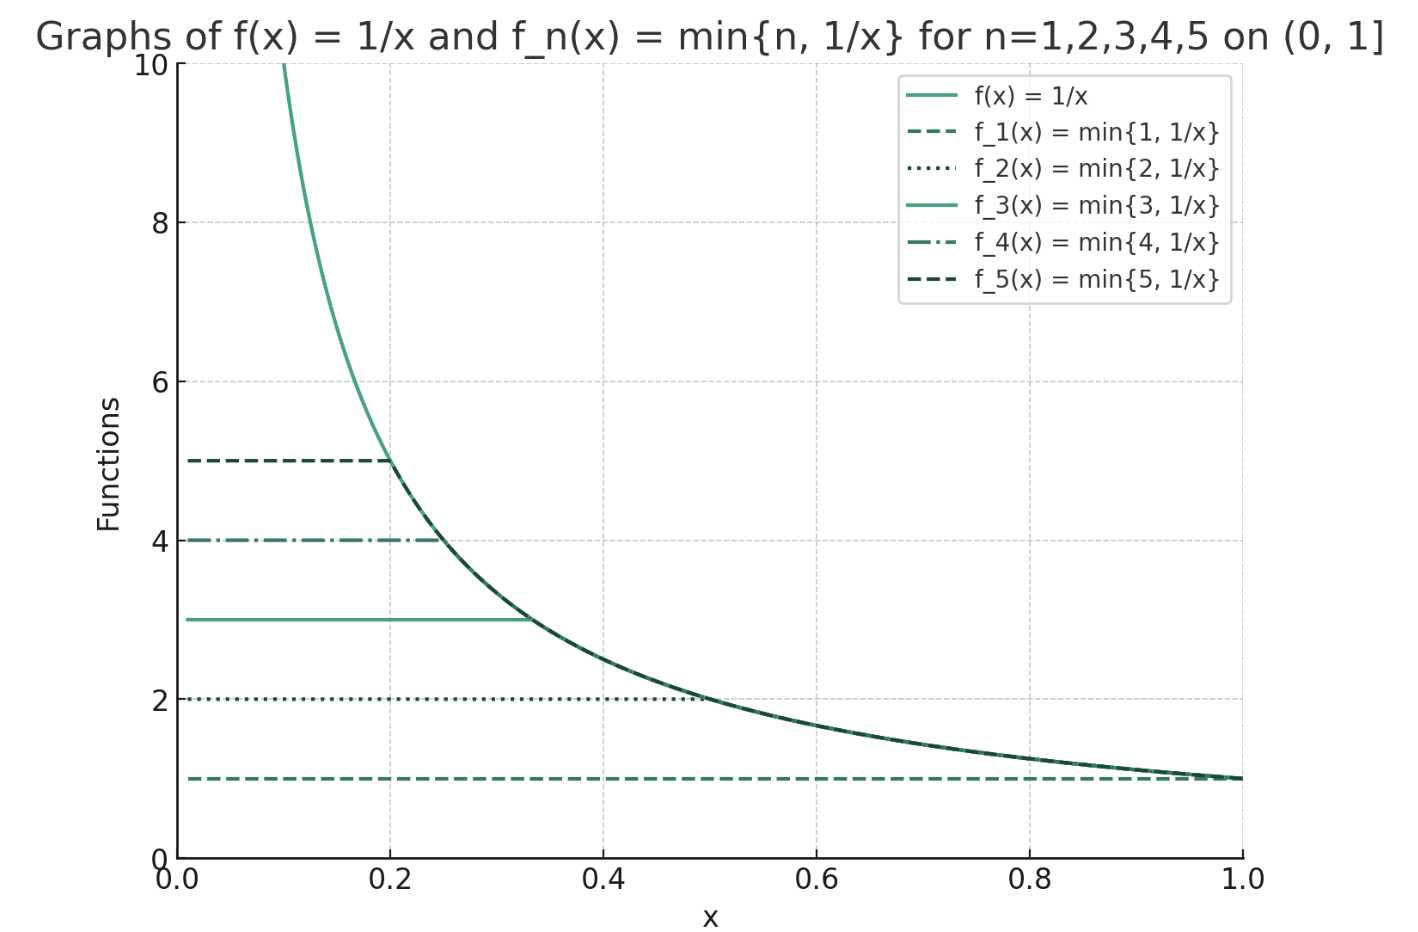
\includegraphics[height=9cm,width=15cm]{pwise converge1.png}
   \end{minipage}
\end{center}
\end{Example}
\begin{Example}{\textbf{(Unbounded functions pointwise converge to bounded function)}}{}
\begin{align*}
X=\R,f_n(x)=\frac{1}{n}x
\end{align*}
The limit function is $f(x)=0$
\begin{center}
   \begin{minipage}{0.9\linewidth}  
       \centering  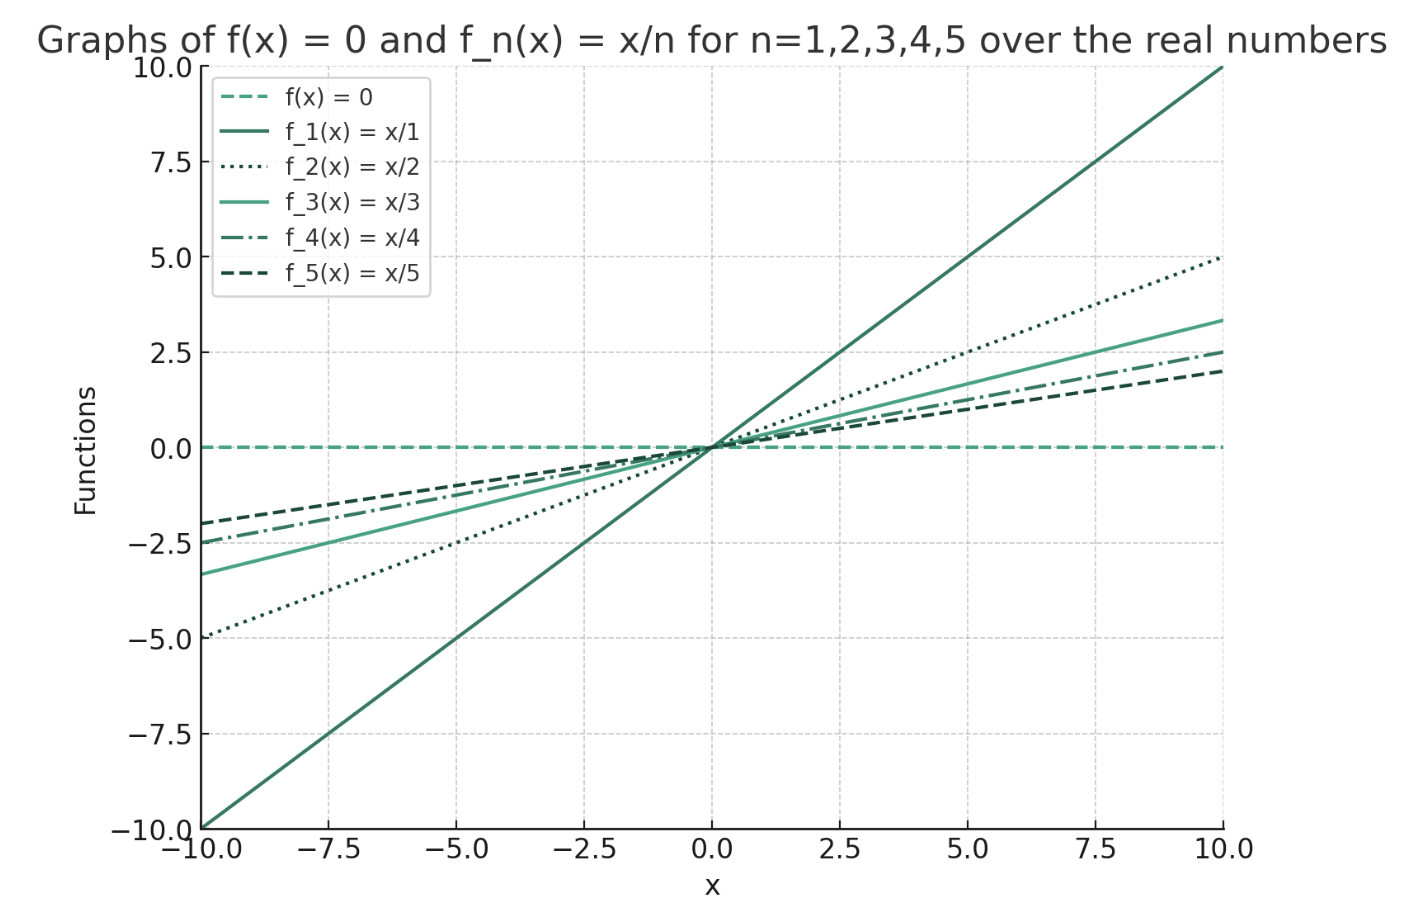
\includegraphics[height=7cm,width=15cm]{pwise converge2.png}
   \end{minipage}
\end{center}
\end{Example}
\end{mdframed} 
\begin{mdframed}
As pointed out earlier, if $f:X\rightarrow (Y,d)$ is bounded and $g:X\rightarrow (Y,d)$ is unbounded, then $d_{\infty}(f,g)=\infty$. This means that if $Y$ is unbounded, the uniform metric $d_{\infty}$ is extended on $X^Y$. For this, it is necessary to develop some basic fact concerning extended metric space.\\

Suppose $(X,d)$ is an extended metric space. If we define $\sim$ on $X$ by $x \sim y\iff  d(x,y)<\infty$, then $\sim $ is an equivalence relation. We say each equivalence class is a \textbf{galaxy} of $(X,d)$. Suppose $T$ is the collection of the galaxies of $(X,d)$. For each $\mathcal{T} \in T$, the space $(\mathcal{T},d)$ is just a metric space.\\

It is easy to see that the way we induce topology from metric space is still valid if the metric is extended. That is 
\begin{align*}
  \tau=\set{Z \in X: \forall z \in Z, \exists \epsilon ,B_\epsilon (z)\subseteq Z}
\end{align*}
is still a topology, even though $d$ is an extended metric on $X$.\\

We can verify that a set $Y$ in $X$ is open if and only if for all  $\mathcal{T} \in T$, the set $Y \cap \mathcal{T}$ is open, and the set $Y$ in $X$ is closed if and only if all convergent sequences $y_n$ in  $Y$ converge to points in $Y$. \\
\end{mdframed}
\begin{mdframed}
Now, suppose we are given an arbitrary set  $X$ and a complete metric space  $(\overline{Y},d)$, and on $X^{\overline{Y}}$, we define the uniform metric  $d_{\infty}$. We say a set $\mathcal{F}\subseteq X^{\overline{Y}}$ of functions is \textbf{closed under uniform convergence} if  for all uniform convergent sequence $f_n \subseteq \mathcal{F}$, the limit function $f$ is also in  $\mathcal{F}$. There are justified reasons for us to give the premise that $\overline{Y}$ is complete prior to the definition of the term \textbf{closed under uniform convergence}. One reason is that by \myref{Theorem}{Tsof}, if $Y$ is not complete, then the extended metric space  $(X^Y,d_{\infty})$ is also not complete, which implies the possibility a Cauchy sequence $f_n$ in  $X^Y$ converge to a function $f \in X^{\overline{Y}} \setminus X^Y$ where $\overline{Y}$ is the completion of  $Y$. For instance, if we let $Y=\R\setminus \set{1}$ where $X=\R$, and let $f_n(x)=\begin{cases}
  0& \text{ if  }x\neq 0\\
  1+\frac{1}{n}& \text{ if $x=0$ }
\end{cases}\in Y$, we see that the set $\mathcal{F}=\set{f_n:n\inn}$ is "closed under uniform convergence" in the context of $X^Y$, but when in fact $f_n$ uniformly converge to  $f(x)=\begin{cases}
  0& \text{ if  }x\neq 0\\
  1& \text{ if $x=0$ }
\end{cases}$ which is not in $\mathcal{F}$. This awkward usage of words can be solved if we define the term  \textbf{closed under uniform convergence} after the premise that $Y$ is complete.\\

Now, given a set of functions $\mathcal{F}\subseteq X^{\overline{Y}}$, one can verify that 
\begin{align*}
  \mathcal{F}\text{ is closed under uniform convergence }&\iff (\mathcal{F},d_{\infty})\text{ is complete }\\
&\iff \mathcal{F}\text{ is closed with respect to $(X^{\overline{Y}},d_{\infty})$ }
\end{align*}
Let $\mathcal{G}$ be a galaxy of $(X^{\overline{Y}},d_{\infty})$. With multiple ways, we can verify that $\mathcal{G}$ is closed with respect to $(X^{\overline{Y}},d_{\infty})$. Then, acknowledging the space of bounded functions $B(X,\overline{Y})$ is a galaxy of $X^{\overline{Y}}$, we see that $B(X,\overline{Y})$ is closed under uniform convergence. The statement that $B(X,\overline{Y})$ is closed under uniform convergence, although already "proved" before as we pointed out the limit of uniform convergent sequence of bounded functions must be bounded, is now in fact actually proved in the sense the term "closed under uniform convergence" is formally given a satisfying definition.
\end{mdframed}
\section{Arzelà–Ascoli Theorem}
\begin{mdframed}
Given a topological space $(X,\tau)$ and a metric space $(Y,d)$, let $\mathcal{F}$ be a collection of functions from $X$ to $Y$. We say $\mathcal{F}$ is \textbf{equicontinuous} if for all $\epsilon $ and for all $x \in X$ there exists a neighborhood $U_x$ around  $x$ such that 
\begin{align*}
\forall y \in U_x, \forall f \in \mathcal{F}, d_Y\big(f(x),f(y) \big)<\epsilon 
\end{align*}
\end{mdframed}
\begin{theorem}
\textbf{(Arzelà–Ascoli theorem)} Given a compact metric space $(X,d_X)$, let $\mathcal{C}(X)$ denote the set of complex-valued continuous function on $X$. Let $\mathcal{F}$ be a subset of $\mathcal{C}(X)$. 
\begin{align*}
\mathcal{F}\text{ is compact in metric space }\big(\mathcal{C}(X),d_{\infty} \big)\iff  \mathcal{F}\text{ is equicontinous and pointwise bounded }
\end{align*}
\end{theorem}
\begin{proof}
$(\longleftarrow)$\\

Let $f_n$ be a sequence in $\mathcal{F}$. To prove $\mathcal{F}$ is compact in $\big(\mathcal{C}(X),d_{\infty} \big)$, we wish 
\begin{align*}
\vi{\text{ to find a sub-sequence }f_{n_k}\text{ that uniformly converge }}
\end{align*}
Because $X$ is compact, we know $X$ is separable. Let $G=\set{x_k}_{k\inn}$ be a countable dense subset of $(X,d_X)$. Because $\mathcal{F}$ is pointwise bounded, we know 
 \begin{align}
\label{A1}
\bset{f_n(x_k)}_{n\inn}\text{ is bounded for all $k \inn$ }
\end{align}
Then by Bolzano-Weierstrass Theorem, we know there exists a convergent sub-sequence 
\begin{align*}
\bset{f_{g_1(k)}(x_1)}_{k\inn} 
\end{align*}
Notice that $\bset{f_{g_1(k)}(x_2)}_{k\inn}$ is a sub-sequence of $\bset{f_n(x_2)}_{n\inn}$. Then because \myref{Equation}{A1}, we know $\bset{f_{g_1(k)}(x_2)}_{k\inn}$ is bounded. Then again by Bolzano-Weierstrass Theorem, we know there exists a convergent sub-sequence 
\begin{align*}
\bset{f_{g_2\circ g_1(k)}(x_2)}_{k\inn}
\end{align*}
Again, notice that $\bset{f_{g_2\circ g_1(k)}(x_3)}$ is a sub-sequence of $\bset{f_n(x_3)}_{n\inn}$. Then again because \myref{Equation}{A1}, again by Bolzano-Weierstrass Theorem, we know there exists a convergent sub-sequence 
\begin{align*}
\bset{f_{g_3\circ g_2\circ g_1(k)}(x_3)}_{k\inn}
\end{align*}
Repeatedly do such, we see 
\begin{align*}
\begin{matrix} 
  f_{g_1(1)}(x_1) & f_{g_2\circ g_1 (1)}(x_2) & f_{g_3\circ g_2 \circ  g_1 (1)}(x_3) & \cdots \\
  f_{g_1(2)}(x_1) & f_{g_2\circ g_1 (2)}(x_2) & f_{g_3\circ g_2 \circ  g_1 (2)}(x_3) & \cdots \\
  f_{g_1(3)}(x_1) & f_{g_2\circ g_1 (3)}(x_2) & f_{g_3\circ g_2 \circ  g_1 (3)}(x_3) & \cdots \\
  \vdots &\vdots &\vdots & \\
  \lim_{k\to \infty } f_{g_1(k)}(x_1) &\lim_{k\to \infty } f_{g_2\circ g_1(k)}(x_2) &\lim_{k\to \infty } f_{g_3\circ g_2\circ g_1(k)}(x_3) \in Y
\end{matrix}
\end{align*}
Now, let 
\begin{align*}
n_k=g_k\circ \cdots \circ  g_1(k)
\end{align*}
Then, we see 
\begin{align*}
\forall m \inn, n_k\text{ is eventually a sub-sequence of }g_m\circ \dots \circ  g_1(k)
\end{align*}
Then we see 
\begin{align*}
\forall j\inn, f_{n_k}(x_j)\to \lim_{k\to \infty}f_{g_j\circ \cdots \circ  g_1(k)}(x_k)\text{ as $k \to \infty$ }
\end{align*}
We claim 
\begin{align*}
\vi{f_{n_k}\text{ uniformly converge }}
\end{align*}
Fix $\epsilon$. We wish  
 \begin{align*}
\vi{\text{ to find }K\inn\text{ such that }\forall k,l>K, \forall x \in X, \abso{f_{n_k}(x)-f_{n_l}(x)}<\epsilon  }
\end{align*}
Because $\mathcal{F}$ is equicontinuous and $\set{f_{n_k}}_{k \inn}\subseteq \mathcal{F}$, we know 
\begin{align}
\label{A2}
\exists \delta , \forall k \inn, \forall x,y \in X , d_X(x,y)<\delta \implies \abso{f_{n_k}(x)-f_{n_k}(y)}<\frac{\epsilon}{3}
\end{align}
Fix such $\delta$. Now, because 
 \begin{align*}
f_{n_j}(x_p)\text{ converge as $j\to \infty$ for each fixed $p\inn$}
\end{align*}
For each fixed $p\inn$, we can let $N_p$ satisfy 
 \begin{align}
  \label{A3}
\forall k,l>N_p, \abso{f_{n_k}(x_p)-f_{n_l}(x_p)}<\frac{\epsilon}{3}
\end{align}
Because $G=\set{x_k}_{k\inn}$ is dense (See the statement above \myref{Equation}{A1}, the statement contains the definition of $G$), we see that 
\begin{align*}
\bset{B_{\delta}(x_k):k\inn}\text{ is an open cover of $(X,d_X)$ }
\end{align*}
Recall by premise that $(X,d_X)$ is compact. Then we know 
\begin{align}
\label{A4}
\text{ there exists a finite set $Q$ of natural number such that $\bset{B_\delta (x_k):k\in Q}$ is an open cover } 
\end{align}
We claim 
\begin{align}
\label{A5}
  \vi{K=\max_{q \in Q}N_q\text{ where $N_q$ is defined by}}\text{ \myref{Equation}{A3}}\vi{\text{ works. }} 
\end{align}
Fix $k,l>K$ and $x \in X$. We wish 
\begin{align*}
\vi{\text{ to prove }\abso{f_{n_k}(x)-f_{n_l}(x)}<\epsilon }
\end{align*}
Because $\bset{B_{\delta}(x_k):k \in Q}$ is an open cover (We create this in \myref{Equation}{A4} from the compactness of $X$), we know there exists $i\in Q$ such that 
\begin{align*}
d_X(x_i,x)<\delta
\end{align*}
By \myref{Equation}{A2} we know 
\begin{align}
\label{A6}
\abso{f_{n_k}(x)-f_{n_k}(x_i)}<\frac{\epsilon}{3}\text{ and }\abso{f_{n_l}(x)-f_{n_l}(x_i)}<\frac{\epsilon}{3}
\end{align}
From the definition of $K$ (\myref{Equation}{A5} and \myref{Equation}{A3}), we know 
\begin{align}
\label{A7}
\abso{f_{n_k}(x_i)-f_{n_l}(x_i)}<\frac{\epsilon}{3}
\end{align}
Then from \myref{Inequality}{A6} and \myref{Inequality}{A7}, we see 
\begin{align*}
\abso{f_{n_k}(x)-f_{n_l}(x)}\leq \abso{f_{n_k}(x)-f_{n_k}(x_i)}+\abso{f_{n_k}(x_i)-f_{n_l}(x_i)}+\abso{f_{n_l}(x_i)-f_{n_l}(x)}<\epsilon \vdone
\end{align*}


 
\end{proof} 
\section{The Stone-Weierstrass Theorem}
\section{Contraction Mapping Theorem}
\chapter{Calculus}

\section{Equivalent Definitions for Riemann Integral}
\begin{mdframed}
In this section, we will give a principal Theorem (\myref{Theorem}{1}) that can serve as a lemma to prove the equivalency of multiple different definitions of Riemann integral on a compact interval. With this approach, we shall diminish the trouble of getting through miscellaneous minor definitions, where they are all equivalent, with only the difference of taking different tags and partitions of certain pattern, which solely serve as a pedagogical tool to give students a concrete idea of integration.\\

A caveat will be made clear here: this section concern only the proper Riemann Integral. That is, we only consider the integration of a function bounded on a compact interval. For a treatment of inproper integral, see \myref{Section}{s1}.\\

In this section, by a \textbf{partition} $P$ of $[a,b]$, we mean a finite set of values $P=\set{a=x_0 \leq  x_1 \leq  \cdots \leq  x_{n_P-1} \leq x_{n_P} =b}$. We say the partition $P'$ is \textbf{finer} than $P$ if $P\subseteq P'$. Given a partition $P$, we put
\begin{align*}
\begin{cases}  
M_i=\sup_{[x_{i-1},x_i]} f(x)\\
m_i=\inf_{[x_{i-1},x_i]}f(x)
\end{cases}\text{and }\begin{cases}
  U(P,f)=\sum_{i=1}^{n_P} M_i \Delta x_i\\
  L(P,f)=\sum_{i=1}^{n_P}m_i\Delta x_i
\end{cases}\text{ where }\Delta x_i= x_i-x_{i-1}
\end{align*}
We shall write $n$ instead of $n_P$ if no confusion will be made.\\


The word \textbf{norm of partition} $\norm{P}$ is defined by $\max_{1\leq i\leq n} \Delta x_i$. We say $U(P,f)$ is an \textbf{upper sum} of $f$. We say the \textbf{upper integral} $\overline{\int_a^b}fdx$ of $f$ on $[a,b]$ is $\inf_P U(P,f)$ where the infimum run through all partitions $P$ of $[a,b]$. The \textbf{lower integral} $\underline{\int_a^b}fdx$ is defined similarly. We say a function $f$ is \textbf{integrable} on $[a,b]$ if   $\overline{\int_a^b}fdx=\underline{\int_a^b}fdx$.\\

Give close attention to the setting that $P$ is finite. This is crucial for making the integration operation possible, since if  $P$ is countable and we define $U(P,f)$ by taking limits for sums, the order of addition can make a difference if the sum does not converge absolutely. This fact is backed by Riemann Rearrangement Theorem  (\myref{Theorem}{t4}), of which we will later give a proof.
\end{mdframed}
\begin{theorem}
\label{1}
\textbf{(Principal for Proving Equivalency of Definitions for Riemann Integral)} 
\begin{align*}
\int_a^b fdx\inr \iff  \forall \set{P_k} : \norm{P_k}\to 0, U(P_k,f)-L(P_k,f)\to 0
\end{align*}
\end{theorem}
\begin{proof}
From right to left is obvious. We prove only 
\begin{align*}
  \vi{\int_a^b fdx\inr \implies   \forall \set{P_k} : \norm{P_k}\to 0, U(P_k,f)-L(P_k,f)\to 0}
\end{align*}
Fix $\epsilon $. We wish to find a positive number $\beta \inr^+$ such that $\forall P: \norm{P}\leq \beta , U(P,f)-L(P,f)<\epsilon $. Because $\int_a^b fdx \inr$, we can let $W$ be a partition such that 
\begin{align*}
U(W,f)-L(W,f)<\frac{\epsilon}{2}
\end{align*}
Let $W=\set{a=x_0^*,x_1^*,\dots ,x_{n_W}^*=b}$, and let $J=\set{1,\dots ,n_W}$ be the set of indices of $W$. Suppose
\begin{align}
\label{e1}
L= \max_{1\leq j\leq n_W-1} \big(\sup_{[x_{j-1}^*,x_{j+1}^*]} f(x)- \inf_{[x_{j-1}^*,x_{j+1}^*]} f(x) \big)
\end{align}
Notice that if $L=0$, then  $f$ must be constant and the proof become trivial, so we can assume $L>0$. We claim that 
\begin{align*}
L\beta n_W\leq \frac{\epsilon}{2}\text{ and }\beta < \min_{j \in J}\Delta x_j
\end{align*}
suffice so that $\forall P:\norm{P}\leq \beta , U(P,f)-L(P,f)<\epsilon $. Let $C= \min_{j \in J}\Delta x_j$. In other words, we now reduce the problem into proving 
\begin{align*}
  \vi{ \norm{P} \leq \min \set{\frac{\epsilon }{2Ln_W },C} \implies U(P,f)-L(P,f)<\epsilon }
\end{align*}
Let $I=\set{1,\dots , n_P}$ be the set of indices for $P$. Suppose 
\begin{align*}
P=\set{a=x_0,x_1,\dots ,x_{n_P}=b}
\end{align*}
We partition $I$ into 
\begin{align*}
\begin{cases}
  A=\bset{i \in I : \exists j \in J,  [x_{i-1},x_i]\subseteq [x_{j-1}^*,x_j^*]}\\
  B=I \setminus  A
\end{cases}
\end{align*}
We now have 
\begin{align}
\label{e2}
U(P,f)-L(P,f)= \sum_{i \in A} \big(M_i-m_i \big) \Delta x_i +\sum_{i \in B} \big(M_i-m_i \big)\Delta x_i
\end{align}
Because for each $i\in A$, there is a unique corresponding $j \in J$ such that $[x_{i-1},x_i] \subseteq [x_{j-1}^*,x_j^*]$, we have 
\begin{align}
  \label{e3}
\sum_{i \in A} \big( M_i-m_i\big) \Delta x_i \leq \sum_{j \in J} \big(M_j^W-m_j^W \big) \Delta x_j^* = U(W,f)-L(W,f)< \frac{\epsilon}{2}
\end{align}
Because $\norm{P}\leq C=\min_{j \in J} \Delta x_j$, we know for each distinct $i \in B$, there exists a distinct $ j \in J$ such that $[x_{i-1},x_i]\subseteq [x_{j-1}^*, x_{j+1}^*]$, so by definition of $L$  (\myref{Equation}{e1}), we have 
\begin{align}
\label{e4}
\sum_{i \in B} \big(M_i-m_i \big) \Delta x_i \leq L\sum_{i \in B} \Delta x_i \leq L n_W \norm{P} \leq \frac{\epsilon }{2} 
\end{align}
Combining  \myref{Equation}{e2}, \myref{Equation}{e3} and \myref{Equation}{e4}, we now see 
\begin{align*}
U(P,f)-L(P,f) <\epsilon \vdone
\end{align*}
\end{proof}
\begin{mdframed}
Recall that we say a series $\sum_{n=1}^\infty a_n$ \textbf{absolutely converge} if $\sum_{n=1}^\infty \abso{a_n} $ converge. We can show that a series converges if it absolutely converges by proving it is Cauchy. In this section, by a \textbf{permutation on $\N$}, we mean a bijective function $\sigma$ from $\N$ to $\N$. Another two important terminologies are the followings. We say that $\sum_{n=1}^\infty a_n$ \textbf{unconditionally converge} if for all permutation $\sigma:\N\rightarrow \N$, the series $\sum_{n=1}^\infty a_{\sigma(n)}$ converge to the same number. We say $\sum_{n=1}^\infty a_n$ \textbf{conditionally converge} if it converge but not unconditionally.\\

In our treatment, Riemann Rearrangement Theorem will be split into 4 parts. The summary is at \myref{Theorem}{t4}. The first part (\myref{Theorem}{2}) states that the limit an absolutely convergent series remain the same under any permutations. The proof for the first part (\myref{Theorem}{2}) may seem technical, but the essence is quite easy to remember. Just "see" that 
\begin{align*}
  \abso{\sum_{k=1}^\infty a_{\sigma (k)}-L}&\leq \abso{\sum_{i<M}a_i -L + \sum_{i\geq M}a_i}\\
&\leq \abso{\sum_{i<M}a_i-L }+\sum_{i\geq M} \abso{a_i} \to 0 \text{ as $M\to 0$ }
\end{align*}
\end{mdframed}
\begin{theorem}
\label{2}
\textbf{(Riemann Rearrangement Theorem, Part 1)}  
\begin{align*}
\sum_{k=1}^\infty a_k \text{ absolutely converge }\implies  \sum_{k=1}^\infty a_k \text{ unconditionally converge }
\end{align*}
\end{theorem}
\begin{proof}
Suppose $\sum_{k=1}^\infty \abso{x_k}$ converge. Let $\sum_{k=1}^\infty x_k=L$. Fix permutation $\sigma :\N\rightarrow \N$. We wish to prove 
\begin{align*}
  \vi{\sum_{k=1}^\infty x_{\sigma(k)}=L}
\end{align*}
Fix $\epsilon $. We reduce the problem into  
 \begin{align*}
   \vi{\text{ finding $N$ such that }\forall n>N, \abso{\sum_{k=1}^n x_{\sigma (k)}- L} <\epsilon }
\end{align*}
Because both $\sum_{k=1}^\infty x_k$ and $\sum_{k=1}^\infty \abso{x_k}$ converge by premise. We know there exists $M$ such that 
\begin{align}
\label{e5}
  \forall n>M, \abso{\sum_{k=1}^n x_k -L}<\frac{\epsilon}{2}\text{ and } \sum_{k=n}^\infty \abso{x_k}<\frac{\epsilon}{2}
\end{align}
Let 
\begin{align*}
I=\sigma^{-1}\big(\set{1,\dots ,M} \big)\text{ and }N=\max I
\end{align*}
We claim 
\begin{align*}
\vi{\text{ such $N$ works }}
\end{align*}
To prove our claim, fix $n>N$. We wish to show 
 \begin{align*}
   \vi{\abso{\sum_{k=1}^n x_{\sigma (k)}-L}<\epsilon }
\end{align*}
Let $I_n=\set{1,\dots , n}$. Observe that 
\begin{align}
\label{e6}
\abso{\sum_{k=1}^n x_{\sigma(k)}-L}&= \abso{\sum_{k \in I_n \setminus I} x_{\sigma (k)}+ \sum_{k \in I} x_{\sigma (k)} - L }
\end{align}
Notice that $k \not \in I \implies  \sigma (k)>M$. Then by definition of $M$  (\myref{Equation}{e5}), we have
\begin{align}
  \label{e7}
\abso{\sum_{k \in I_n \setminus I} x_{\sigma (k)} }\leq \sum_{k \in I_n \setminus  I} \abso{x_{\sigma(k)}}\leq \sum_{j>M}^\infty \abso{x_j}< \frac{\epsilon}{2}
\end{align}
Notice that $\sigma [I]=\set{1,\dots , M}$. Then also by definition of $M$  (\myref{Equation}{e5}), we have 
\begin{align}
\label{e8}
\abso{\sum_{k \in I}x_{\sigma(k)}- L}= \abso{\sum_{j=1}^M x_j-L}< \frac{\epsilon}{2}
\end{align}
Then by inequalities \myref{Equation}{e6}, \myref{Equation}{e7} and \myref{Equation}{e8}, we now have 
\begin{align*}
\abso{\sum_{k=1}^n a_{\sigma(k)}-L} &= \abso{\sum_{k \in I_n \setminus I}x_{\sigma(k)} + \sum_{k \in I} x_{\sigma(k)}-L}\\
&\leq \abso{\sum_{k \in I_n \setminus I}x_{\sigma(k)}}+\abso{\sum_{k \in I} x_{\sigma(k)}-L} \\
&< \frac{\epsilon }{2}+\frac{\epsilon}{2}=\epsilon \vdone 
\end{align*}
\end{proof}
\begin{mdframed}
The second, third and forth parts (\myref{Theorem}{t1}, \myref{Theorem}{t2} and \myref{Theorem}{t3}), respectively states that if a series converge but not absolutely, then the limit value can be changed to any real number, infinite, negative infinite and even jumping-ly diverges.\\

The detail of the proof is very tedious and cumbersome, while the essence is easy to understand. The only two tools for proving \myref{Theorem}{t1}, \myref{Theorem}{t2} and \myref{Corollary}{t3}, is \myref{Lemma}{l1} and the fact $\sum a_k\to L \implies a_k\to 0$. If any part of the proof can be considered interesting, I believe it lies in that of \myref{Lemma}{l1}, where one split the series $\sum a_k$ into two $\sum a_k^+,\sum a_k^-$, and shows that they must both diverge. 
\end{mdframed}
\begin{lemma}
\label{l1}
\textbf{(Intrinsic Structure of Series that Converge but not Absolutely)} Let $f^+:\N\rightarrow \N$ and $f^-:\N\rightarrow \N$ satisfy that $\set{a_{f^+(n)}}$ contain all and only positive terms of $\set{a_n}$ and $\set{a_{f^-(n)}}$ contain all and only negative terms. If $\sum_{k=1}^\infty a_k$ converge but not absolutely, then for each $\alpha \inr^+$ and $n\inn$, there exists  $u_n>n$ and $t_n>n$ such that 
\begin{align*}
\sum_{n\leq k\leq u_n} a_{f^+(k)}>\alpha \text{ and }\sum_{n\leq k\leq t_n}a_{f^-(k)}<-\alpha 
\end{align*}
\end{lemma}
\begin{proof}
Let $a_n^+=\max \set{0,a_n}$ and $a_n^-=\min \set{0,a_n}$. It is easy to check $\forall n\inn, a_n=a_n^++a_n^-$. Because $\sum_{k=1}^\infty a_k$ converge but not absolutely, we know 
\begin{align}
\label{e9}
\begin{cases}
  \sum_{k=1}^\infty a_k^+\to\infty\\
  \sum_{k=1}^\infty a_k^-\to-\infty
\end{cases}
\end{align}
This is true because if both of them converge then $\sum_{k=1}^\infty \abso{a_k}$ converges and if only one of them converge them $\sum_{k=1}^\infty a_k$ diverges.\\


Because of  \myref{Equation}{e9}, we know 
\begin{align*}
\begin{cases}
  \sum_{k=1}^\infty a_{f^+(k)}\to \infty\\
  \sum_{k=1}^\infty a_{f^-(k)}\to -\infty
\end{cases}
\end{align*}
The result then follow, since 
\begin{align*}
\forall n\inn, \sum_{k\geq n}a_{f^+(k)}\nearrow \infty \text{ and }\sum_{k\geq n}a_{f^-(k)}\searrow -\infty
\end{align*}
\end{proof}
\begin{theorem}
\label{t1}
\textbf{(Riemann Rearrangement Theorem, Part 2)} If $\sum_{k=1}^\infty a_k$ converge but not absolutely, then there exists permutations $\sigma_{\infty}, \sigma_{-\infty}:\N\rightarrow \N$ such that $\sum_{k=1}^\infty a_{\sigma_\infty(k)}\to\infty$ and $\sum_{k=1}^\infty a_{\sigma_{-\infty}(k)}\to-\infty$. 
\end{theorem}
\begin{proof}
We wish
\begin{align*}
\vi{\text{ to construct $\sigma_{\infty}:\N\rightarrow \N$ such that  $\sum_{k=1}^\infty a_{\sigma_{\infty}(k)}\to\infty$}}
\end{align*}
Using \myref{Lemma}{l1}, construct $\sigma_{\infty}:\N\rightarrow \N$ as follows. Let $p_n$ be a sequence of natural number such that for each $n\inn$, $p_{n+1}$ is the smallest natural number such that 
\begin{align}
\label{e10}
\sum_{k=p_n+1}^{p_{n+1}} a_{f^+(k)}> 3\text{ and }p_1=0
\end{align}
Similarly, let $q_n$ be a sequence of natural number such that for each $n\inn,q_{n+1}$ is the smallest natural number such that 
\begin{align}
\label{e11}
\sum_{k=q_n+1}^{q_{n+1}}a_{f^-(k)}<-1\text{ and }q_1=0
\end{align}
Notice that the definition of $p_n$ and  $q_n$ (\myref{Equation}{e10}, \myref{Equation}{e11}) are done recursively. Now, recursively define $\sigma_{\infty}$ to follow the order
\begin{align*}
&f^+(p_1+1),\dots,f^+(p_2),f^-(q_1+1),\dots ,f^-(q_2)\\
  \longrightarrow &  f^+(p_2+1),\dots ,f^+(p_3),f^-(q_2+1),\dots ,f^-(q_3),f^+(p_3+1),\dots 
\end{align*}
If there exists  $k\inn$ such that $a_k=0$, which is not in the range $f^+[\N]\cup f^-[\N]$, we can merge these zero term into our $\sigma_{\infty}$ by putting them in terms of even order. This way, our $\sigma_{\infty}$ then become bijecetive, a permutation.\\

We claim 
\begin{align*}
  \vi{\text{ such }\sigma_{\infty}\text{ works }}
\end{align*}
Recall the definition of $p_n$ (\myref{Equation}{e10}) is that for each  $n\inn,p_{n+1}$ is the smallest natural number such that
\begin{align*}
\sum_{k=p_{n}+1}^{p_{n+1}}a_{f^+(k)}>3 
\end{align*}
Also recall the similarly defined $q_n$. This tell us 
\begin{align*}
\sum_{k=p_n+q_n+1}^{p_{n+1}+q_{n+1}}a_{\sigma_{\infty}(k)}\to 2\text{ as $n\to \infty$ }
\end{align*}
where 
\begin{align*}
\sum_{k=p_n+q_n+1}^{p_{n+1}+q_n}a_{\sigma_\infty(k)}\to 3\text{ and }\sum_{k=p_{n+1}+q_n+1}^{p_{n+1}+q_{n+1}}a_{\sigma_\infty(k)}\to -1\text{ as $n \to \infty$ }
\end{align*}
With this, it is easy to verify $\sum_{k=1}^\infty a_{\sigma_{\infty}(k)} \to \infty\vdone$. The construction of $\sigma_{-\infty}$ and the proof for its validity is done similarly. 
\end{proof}
\begin{theorem}
\label{t2}
\textbf{(Riemann Rearrangement Theorem, Part 3)} If $\sum_{k=1}^\infty a_k$ converges but not absolutely, then for all $[L,M]\subseteq \R$, there exists a permutation $\sigma:\N\rightarrow \N$ such that $\liminf_{n\to\infty} \sum_{k=1}^n a_{\sigma(k)}=L\text{ and }\limsup_{n\to\infty} \sum_{k=1}^n a_{\sigma(k)}=M$.
\end{theorem}
\begin{proof}
We wish 
\begin{align*}
\vi{\text{ to construct a working $\sigma$ }}
\end{align*}
The construction of $\sigma$ is similar to that of $\sigma_{\infty}$ in \myref{Theorem}{t1}. WOLG, let $M>0$. Let $p_1=0$, and let  $p_2$ be the smallest natural number such that 
 \begin{align*}
\sum_{k=1}^{p_2}a_{f^+(k)}>M\text{ and }p_1=0
\end{align*}
Next, define $q_1=0$ and let $q_2$ be the smallest natural number such that 
 \begin{align*}
\sum_{k=1}^{p_2}a_{f^+(k)}+\sum_{k=1}^{q_2} a_{f^-(k)}<L
\end{align*}
Then, let $p_3$ be the smallest natural number such that 
\begin{align*}
\sum_{k=1}^{p_3}a_{f^+(k)}+\sum_{k=1}^{q_2}a_{f^-(k)}>M
\end{align*}
Recursively do such. We get two sequences $\set{p_n},\set{q_n}$ of natural number such that for all $n\inn,p_{n+1}$ is the smallest natural number such that 
\begin{align*}
\sum_{k=1}^{p_{n+1}} a_{f^+(k)} +\sum_{k=1}^{q_n}a_{f^-(k)}>M
\end{align*}
and for all $n\inn,q_{n+1}$ is the smallest natural number such that 
\begin{align*}
\sum_{k=1}^{p_{n+1}}a_{f^+(k)} + \sum_{k=1}^{q_{n+1}} a_{f^-(k)}<L
\end{align*}
Them, recursively define $\sigma$ to follow the order 
\begin{align*}
&f^+(p_1+1),\dots,f^+(p_2),f^-(q_1+1),\dots ,f^-(q_2)\\
  \longrightarrow &  f^+(p_2+1),\dots ,f^+(p_3),f^-(q_2+1),\dots ,f^-(q_3),f^+(p_3+1),\dots 
\end{align*}
Again, merge in the zero terms like in   \myref{Theorem}{t1}. The proof for the claim  \vi{such $\sigma$ works } is easy to verify knowing $a_{\sigma(k)}\to 0\vdone$ 
\end{proof}
\begin{corollary}
\label{t3}
\textbf{(Riemann Rearrangement Theorem, Part 4)} If $\sum_{k=1}^\infty a_k$ converges but not absolutely, then for all $L \inr$, there exists a permutation $\sigma$ such that $\sum_{k=1}^\infty a_{\sigma(k)}=L$
\end{corollary}
\begin{theorem}
\label{t4}
\textbf{(Summary of Riemann Rearrangement Theorem)} If $\sum_{k=1}^\infty a_k$ converge, then 
\begin{align*}
\sum_{k=1}^\infty a_k\text{ absolutely converges }\iff  \sum_{k=1}^\infty a_k\text{ unconditionally converges }
\end{align*}
\end{theorem}
\begin{proof}
$(\longrightarrow)$\\

This is \myref{Theorem}{2}.\\

$(\longleftarrow)$\\

The fact that the contraposition of this  statement is true is implied by any of \myref{Theorem}{t1}, \myref{Theorem}{t2} and \myref{Corollary}{t3}. 
\end{proof}
\section{Product, Quotient and Chain Rule}
\begin{mdframed}
This section concern mostly the computation of actual value of the derivative and integral of function. With this in mind, we first prove the product and quotient rules for derivative of $\R$ to  $\R$ functions taught in most Calculus 1 classes. The proofs for the laws are easy, as it require no ingenious idea but ability to manipulate the limit symbol. However, without philosophical comments, we left an graph for geometric intuition for product rule. There are also graphs for geometric intuition for quotient rule on Internet, but we won't put it here as it require more than subtle work to understand the graph.    
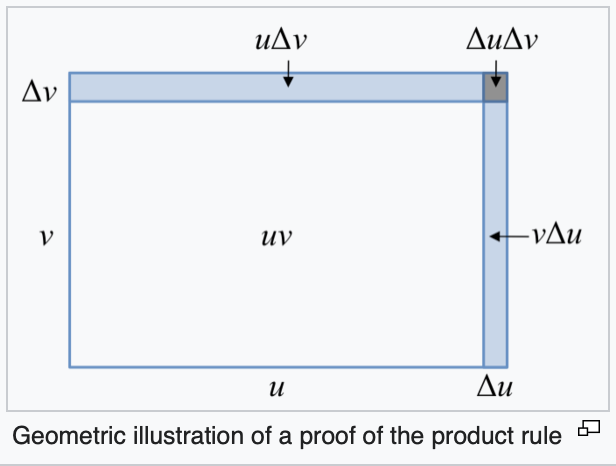
\includegraphics[height=7cm,width=10cm]{product rule.png}
\end{mdframed}
\label{11}
\begin{theorem}
\textbf{(Product Rule and Quotient Rule for Real to Real Function)} Suppose $f$ and $g$ is differentiable at  $x$, and $g'(x)\neq 0$. We have 
\label{3}
\begin{enumerate}[label=(\alph*)]
  \item $(fg)'(x)=f'(x)g(x)+f(x)g'(x)$ (Product Rule)
  \item $(\frac{f}{g})'(x)=\frac{f'(x)g(x)-f(x)g'(x)}{\big(g(x) \big)^2}$ (Quotient Rule)
\end{enumerate}
\end{theorem}
\begin{proof}
Compute 
\begin{align*}
  (fg)'(x)&=\lim_{h\to_0} \frac{f(x+h)g(x+h)-f(x)g(x)}{h}\\
          &=\lim_{h\to 0} \frac{f(x+h)g(x+h)-f(x)g(x+h)+f(x)g(x+h)-f(x)g(x)}{h}\\
          &=\lim_{h\to0} \big(g(x+h) \big) \frac{f(x+h)-f(x)}{h} + \big(f(x) \big) \frac{g(x+h)-g(x)}{h}\\
          &=g(x)f'(x)+f(x)g'(x)
\end{align*}
Compute 
\begin{align*}
  (\frac{f}{g})'(x)&=\lim_{h\to0} \frac{\frac{f(x+h)}{g(x+h)}-\frac{f(x)}{g(x)}}{h}\\
  &=\lim_{h\to0} \frac{f(x+h)g(x)-f(x)g(x+h)}{h g(x+h)g(x)}\\
  &=\lim_{h\to0}\big(\frac{1}{g(x+h)g(x)} \big)\cdot \big(\frac{f(x+h)g(x)-f(x)g(x)+f(x)g(x)-f(x)g(x+h)}{h} \big)\\
  &=\lim_{h\to 0} \Big(\frac{1}{g(x+h)g(x)} \Big) \cdot \Big(\big(g(x) \big) \frac{f(x+h)-f(x)}{h} +\big(f(x) \big) \frac{g(x)-g(x+h)}{h}\Big)\\
  &=\Big(\frac{1}{\big(g(x) \big)^2} \Big)\cdot \Big(\big(g(x)f'(x) \big)-f(x)g'(x) \Big)=\frac{f'(x)g(x)-f(x)g'(x)}{\big(g(x) \big)^2}
\end{align*}
\end{proof}
\begin{mdframed}
  Even a year has past, I can still remember what happened in the first class of Vector Analysis last year. The professor asked: "What is derivative?". A lot of answers emerge, from extremely formal and abstract like $\lim_{h\to 0}\frac{f(x+h)-f(x)}{h}$ to those following geometric intuition like tangent line. Everyone gave a correct answer, but none of them philosophically satisfy the requirement of the question from the professor. Then, he stated: "Derivative is exactly linear approximation", and stated on black board the most general definition:


\end{mdframed}
\begin{definition}
\label{4}
  \textbf{(Definition of Differential)} Given two normed space $V,W$ and an open subset $U\subseteq V$,  we say a function $f:U\rightarrow W$ is \textbf{differentiable at $x$} if there exists a bounded linear operator $A:V\rightarrow W$ such that 
\begin{align*}
\lim_{ h\to 0} \frac{\norm{f(x+h)-f(x)-A(h)}_W}{\norm{h}_V}=0
\end{align*}
and we say the bounded linear map $A$ is the \textbf{(total) derivative} of $f$ at  $x$. 
\end{definition}
\begin{mdframed}
If one put the key words "proof for chain rule" in Google search box, just like the situation in my classes, lots of rigorous proof emerge, but none of them is philosophical satisfying. For this reason, I shall give a proof of chain rule for real to real function based on the concept of linear approximation.\\

In Baby Rudin, derivative of a real to real function $f$ is defined by 
\begin{align*}
f'(a)=\lim_{h\to 0}\frac{f(a+h)-f(a)}{h}
\end{align*}
Immediately from this definition, we can derive a linear approximation $P$ of $f$ at $a$ by setting 
\begin{align*}
P(x)=f(a)+f'(a)(x-a)
\end{align*}
Then, we see if we set $R(x)=f(x)-P(x)$ as the error (or the remainder) of the approximation, then trivially we have the behavior
\begin{align*}
R(x)\to 0\text{ as $x\to a$ }
\end{align*}
what behavior of $R(x)$ that give $P$ the name approximation is 
\begin{align*}
\frac{R(x)}{x-a}\to 0\text{ as }x\to a
\end{align*}
The difference between the two behaviors is symbolically apparent, yet without geometric help, it may be difficult to precisely describe how insignificant the first behavior is compared to the second behavior. For this, observe that any function $g$ that converge to  $f(a)$ at $a$ satisfy the first behavior, yet only a few satisfy the second. One can easily verify that the only linear $\R$ to  $\R$ function that satisfy the second behavior is  $P(x)=f(a)+f'(a)(x-a)$. Geometrically, this means that $R(x)=o(f'(x)dx)$ as $x \to a$.
\label{12}
\end{mdframed}
\begin{theorem}
\textbf{(Chain Rule for $\R$ to $\R$ function)} Suppose $g$ is differentiable at  $a$ and  $f$ is differentiable at  $g(a)$. We have 
\begin{align*}
  (f\circ g)'(a)=f'(g(a))g'(a)
\end{align*}
\end{theorem}
\begin{proof}
Define the remainders $R_{f(g(a))}(x)$ and $R_{g(a)}(x)$ by 
\begin{align*}
\begin{cases}
R_{f(g(a))}(x)=f(x)-f(g(a))-f'(g(a))(x-g(a))\\
R_{g(a)}(x)=g(x)-g(a)-g'(a)(x-a)
\end{cases}
\end{align*}
Compute 
\begin{align}
\label{3.13}
  (f\circ g)'(a)&=\lim_{ x\to a}\frac{f(g(x))-f(g(a))}{x-a}\\
  &=\lim_{x\to a}\frac{R_{f(g(a))}(g(x))+f'(g(a))(g(x)-g(a))}{x-a}
\end{align}
Notice that because $x \to a \implies g(x)\to g(a)$, we have 
\begin{align}
\label{3.12}
\lim_{x\to a} \frac{R_{f(g(a))}(g(x))}{x-a}=\lim_{ x\to a} \frac{R_{f(g(a))}(g(x))}{g(x)-g(a)}\cdot \frac{g(x)-g(a)}{x-a}=0\cdot g'(x)=0
\end{align}
Notice that the above deduction (\myref{Equation}{3.12}) is quite informal for two reasons: First, it may happen that $g(x)=g(a)$ locally. Second, for some reader it may require a mini proof to verify that $\frac{R_{f(g(a))}(g(x))}{g(x)-g(a)}\to 0$ as $x\to a$. These two obstacles for advanced readers should be insignificant.\\

Getting back to \myref{Equation}{3.13}, by \myref{Equation}{3.12}, we now see 
\begin{align*}
  (f\circ g)'(a)=\lim_{x\to a}\frac{f'(g(a))(g(x)-g(a))}{x-a}=f'(g(a))g'(a)
\end{align*}
which finish the proof.
\end{proof}
\section{IVT, EVT and MVT}
\begin{mdframed}
  If one wish to understand most of the Theorems after this section, one must first know MVT, for what an important role it cast in the sections after. Logically prior to MVT is IVT. Yet, unlike MVT involve the intrinsic nature of field and limit structure of $\R$. IVT can be considered as purely topological in the sense that its proof can be stated almost in the language of topology. There are only two facts (the first are purely topological and the second is very close to purely topological) one need to know to prove IVT.\\

First, continuous functions map a connected sets to  connected set. Second, a set in $\R$ is connected if and only if it is an interval.\\

Combining the above two facts, we have the following statement:  
\label{13}
\end{mdframed}
\label{5}
\begin{theorem}
\textbf{(Continuous Real to Real Function Maps Interval to Interval)} as titled.
\end{theorem}
\begin{proof}
Consider the fact a continuous function map connected sets to connected sets and the fact a set in $\R$ is connected if and only if it is an interval.
\end{proof}
\begin{mdframed}
\label{14}
Then, given the necessary constraint (the interval considered is compact) to give the conclusion, we have the famous statement:
\label{6}
\end{mdframed}
\begin{theorem}
\textbf{(IVT)} Given a continuous function $f:[a,b]\to \R$, for each $y$ that lies between $f(a)$ and $f(b)$, there exists $x \in [a,b]$ such that $f(x)=y$.
\end{theorem}
\begin{mdframed}
Given the simplicity of the logical deduction, we shall not give a rigorous proof here. However, one can notice that the interval considered in IVT "must be" compact, otherwise the Theorem is invalid. This constraint is in some sense a showcase how the concept of compact really match  the description of "smallness (bounded) and rigidness (closed)". \\
\label{15}

\label{7}
Compared to IVT, another famous MVT is richer in both the results and the proof. Clearly for a logical and economic purpose, we shall first prove the Cauchy MVT.

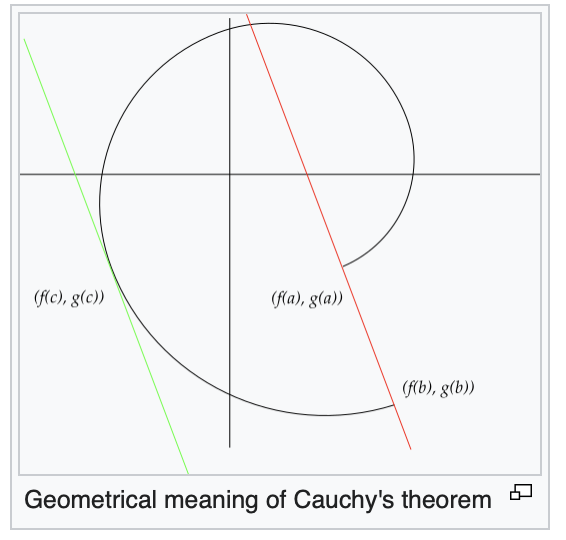
\includegraphics[height=7cm,width=10cm]{CMVT.png}
\end{mdframed}
\begin{theorem}
\label{CMVT}
\textbf{(Cauchy's MVT)} Given a function $f:[a,b]\to \R$ such that  
\begin{enumerate}[label=(\alph*)]
  \item $f,g$ are  differentiable on $(a,b)$
  \item $f,g$ are continuous on $[a,b]$
\end{enumerate}
There exists $x \in (a,b)$ such that 
 \begin{align*}
   \big[f(b)-f(a) \big]g'(x)=\big[g(b)-g(a) \big]f'(x)
\end{align*}
\end{theorem}
\begin{proof}
We wish to find $x \in (a,b)$ such that  
\begin{align*}
\vi{\big[f(b)-f(a)]g'(x)-[g(b)-g(a)]f'(x)=0}
\end{align*}
Define $h$ on  $(a,b)$ by 
\begin{align*}
h(x)=\big[f(b)-f(a)\big]g'(x)-\big[g(b)-g(a)\big]f'(x)
\end{align*}
We reduced our problem into finding $x \in (a,b)$ such that 
\begin{align*}
\vi{h(x)=0}
\end{align*}
Because $f,g$ are both differentiable on  $(a,b)$, we know there exists an anti-derivative $H$ of  $h$ on  $(a,b)$ such that
\begin{align*}
H(x)=\big[f(b) -f(a)\big]g(x)-\big[g(b)-g(a) \big]f(x)
\end{align*}
We have $h=H'$ on  $(a,b)$. This let us reduce our problem into 
\begin{align*}
  \vi{\text{ finding a local extremum of $H$ on  $(a,b)$ }}
\end{align*}
Because $f,g$ are both continuous  on  $[a,b]$, we know $H$ is continuous on $[a,b]$. Then by EVT, we know 
 \begin{align*}
\exists x \in [a,b] , H(x)=\max_{t \in [a,b]}H(t)\text{ and }\exists y \in [a,b], H(y)=\min_{t \in [a,b]}H(t)
\end{align*}
If such $x,y$ is in $(a,b)$, we are done. If not, says that $x,y$ both are on end points $a$ or  $b$. Compute that 
\begin{align*}
H(a)=f(b)g(a)-g(b)f(a)=H(b)
\end{align*}
We see $H$ is constant on  $[a,b]$. Then all points in $(a,b)$ are extremums. $\vdone$
\end{proof}
\begin{corollary}
\label{MVT}
\textbf{(Lagrange's MVT)} Given a function $f:[a,b]\rightarrow \R$ such that 
\begin{enumerate}[label=(\alph*)]
  \item $f$ is differentiable on  $(a,b)$ 
  \item $f$ is continuous on  $[a,b]$
\end{enumerate}
Then there exists $x \in (a,b)$ such that 
\begin{align*}
f'(x)=\frac{f(b)-f(a)}{b-a}
\end{align*}
\end{corollary}
\begin{proof}
Let $g(x)=x$ in Cauchy's MVT (\myref{Theorem}{CMVT}), and we are done.
\end{proof}
\begin{mdframed}
There are two hypotheses in Lagrange's MVT 
\begin{enumerate}[label=(\alph*)]
  \item $f$ is differentiable on $(a,b)$ 
  \item $f$ is continuous on $[a,b]$
\end{enumerate}
They are all necessary. The necessity of differentiablity on $(a,b)$ is clear as shown by the canonical example using absolute value. The necessity of continuity on $[a,b]$ can be shown by the example 
\begin{align*}
f(x)=\begin{cases}
  1& \text{ if $a<x\leq b$ }\\
  0& \text{ if  }x=a
\end{cases}
\end{align*}
\end{mdframed}
\begin{theorem}
\textbf{(First Mean Value Theorem for Definite Integral)} Given a function $f:[a,b]\rightarrow \R$ such that 
\begin{enumerate}[label=(\alph*)]
  \item $f$ is continuous on $(a,b)$
\end{enumerate}
There exists $\xi \in (a,b)$ such that 
\begin{align*}
\int_a^b f(x)dx = f(\xi)\cdot (b-a)
\end{align*}
\end{theorem}
\begin{proof}
We wish 
\begin{align*}
\vi{\text{ to find  }\xi \in (a,b)\text{ such that }f(\xi)=\frac{\int_a^b f(x)dx}{b-a}}
\end{align*}
Define $\tilde{f}:[a,b]\rightarrow \R$ on $[a,b]$ by 
\begin{align}
\label{M1}
\tilde{f}(x)=\begin{cases}
  f(x)& \text{ if $x \in (a,b)$ }\\
  \lim_{t\to a}f(t)& \text{ if $x=a$ }\\
  \lim_{t\to b}f(t)& \text{ if $x=b$ }
\end{cases}
\end{align}
Then, because $\int_a^b f(x)dx=\int_a^b \tilde{f}(x)dx $, we reduce our problem into  
\begin{align*}
\vi{\text{ finding $\xi\in(a,b)$ such that $\tilde{f} (\xi)= \frac{\int_a^b \tilde{f}(x)dx }{b-a}$ }}
\end{align*}
Because $\tilde{f} $ is continuous on $[a,b]$ by definition \myref{Equation}{M1}, by EVT, we know we there exists $\alpha,\beta  \in [a,b]$ such that 
\begin{align}
\label{M4}
\tilde{f} (\alpha )=\inf_{x \in [a,b]}\tilde{f}(x)\text{ and } \tilde{f}(\beta ) =\sup_{x \in[a,b]}\tilde{f}(x) 
\end{align}
WOLG, suppose $\alpha \leq \beta $. Deduce 
\begin{align*}
\tilde{f}(\alpha )= \inf_{x \in [a,b]}\tilde{f}(x)\leq \frac{\int_a^b \tilde{f}(x)dx }{b-a} \leq \sup_{x \in [a,b]}\tilde{f}(x) =\tilde{f}(\beta ) 
\end{align*}
by IVT, we then know there exists $\xi\in [\alpha ,\beta ]$ such that 
\begin{align}
\label{M3}
\exists \xi\in [\alpha ,\beta ], \tilde{f}(\xi)=\frac{\int_a^b \tilde{f}(x)dx }{b-a} 
\end{align}
If $a<\alpha $ and $\beta <b$, our proof is done.\\


If not, notice that if $\tilde{f}(\alpha )=\tilde{f}(\beta )$, then by definition of $\alpha ,\beta $ (\myref{Equation}{M4}), the proof is trivial since $\tilde{f}$ is a constant, so we only have to consider when $\tilde{f}(\alpha )<\tilde{f}(\beta )  $, and we wish to show
\begin{align*}
\vi{\xi \text{ can not happen at $a$ nor $b$ }}
\end{align*}
\As{$\xi=a $, WOLG}. Because $\xi \in [\alpha ,\beta ]$, we know $\alpha =a$. Because $\tilde{f}(\beta )>\tilde{f}(\alpha )  $, we can find $\delta $ such that 
\begin{align}
\label{M5}
\inf_{x \in [\beta  -\delta, \beta  ]}\tilde{f}(x)\geq \frac{\tilde{f}(\alpha )+2\tilde{f}(\beta )  }{3}
\end{align}
We then from \myref{Equation}{M3} see that 
\begin{align}
\label{M6}
\int_a^b \tilde{f}(x)dx=\tilde{f}(\xi)(b-a)=\tilde{f}(\alpha ) (b-a)
\end{align}
Also, we see from definition of $\alpha $ (\myref{Equation}{M4}) and \myref{Equation}{M5} that 
\begin{align}
\int_a^b \tilde{f}(x)dx&=\int_a^{\beta -\delta} \tilde{f}(x)dx + \int_{\beta -\delta}^{\beta  } \tilde{f}(x)dx+\int_{\beta }^{b}\tilde{f}(x)dx \\
&\geq (b -\delta -a) \tilde{f}(\alpha ) + \delta \cdot  \big( \frac{\tilde{f}(\alpha )+2\tilde{f}(\beta )  }{3}\big)\\
&> (b -\delta -a) \tilde{f}(\alpha ) + \delta \cdot  \big( \frac{\tilde{f}(\alpha )+\tilde{f}(\beta )  }{2}\big)\\
&=\tilde{f}(\alpha ) \big(b-a-\frac{\delta}{2} \big) + \tilde{f}(\beta ) \cdot \big( \frac{\delta}{2}\big)
 \label{M7}
\end{align}
Now, from \myref{Equation}{M6} and \myref{Equation}{M7}, we can deduce  
\begin{align*}
\tilde{f}(\alpha )(b-a)> \tilde{f}(\alpha )(b-a-\frac{\delta}{2}) +\tilde{f}(\beta ) \cdot \big(\frac{\delta}{2} \big)
\end{align*}
Then we can deduce
\begin{align*}
\tilde{f}(\alpha )\cdot \big(\frac{\delta}{2} \big)>\tilde{f}(\beta )\cdot \big(\frac{\delta}{2} \big) \tCaC \vdone
\end{align*}
\end{proof}
\begin{theorem}
\textbf{(Second Mean Value Theorem for Definite Integral)} Given functions $G,\phi :[a,b]\rightarrow \R$ such that 
\begin{enumerate}[label=(\alph*)]
  \item $G$ is monotonic
  \item $\phi$ is Riemann-Integrable
\end{enumerate}
Let $G(a^+)=\lim_{t\to a^+}G(t)$ and $G(b^-)=\lim_{t\to b^-}G(t)$. Then there exists $\xi \in (a,b)$ such that 
\begin{align*}
\int_a^b G(t)\phi (t)dt= G(a^+)\int_a^{\xi} \phi(t)dt+G(b^-)\int_\xi^{b}\phi (t)dt
\end{align*}
\end{theorem}
\begin{proof}
Define $f$ on  $[a,b]$ by 
\begin{align*}
f(x)=G(a^+)\int_a^x \phi(t)dt+G(b^-)\int_x^b \phi(t)dt
\end{align*}
We then reduce the problem into 
\begin{align*}
\vi{\text{ finding }\xi \in (a,b)\text{ such that }\int_a^b G(t)\phi (t)dt=f(\xi)}
\end{align*}
By \myref{Theorem}{FTC1}, we know $f$ is continuous on  $[a,b]$. Then by IVT, we can reduce the problem into 
\begin{align*}
\vi{\text{ finding an interval $[c,d]\subseteq (a,b)$ such that }\int_a^b G(t)\phi (t)}\text{ is between $f(c) $ and $f(d)$ }
\end{align*}


Observe that 
\begin{align*}
f(a)=G(b^-)\int_a^b \phi(t)dt\text{ and }f(b)=G(a^+)\int_a^b \phi(t)dt 
\end{align*}




\end{proof}




\section{Computation for Riemann-Stieltjes Integral}
\begin{theorem}
\label{CoV}
\textbf{(Change of Variable)} Given two functions $g,\beta  :[A,B]\rightarrow \R$, a function $\phi: [A,B]\rightarrow [a,b]$ and two functions $f,\alpha :[a,b]\rightarrow \R$ such that 
\begin{enumerate}[label=(\alph*)]
  \item $g = f \circ  \phi $ for all $x \in [a,b]$
  \item $\beta = \alpha  \circ \phi $ for all $x \in [a,b]$ 
  \item $\alpha , \beta  $ increase respectively on $[a,b]$ and $[A,B]$ 
  \item $\phi:[A,B]\rightarrow [a,b]$ is a homeomorphism 
  \item $\int_a^b fd\alpha $ exist
\end{enumerate}
Then 
\begin{align*}
\int_A^B g d\beta  =\int_a^b fd\alpha \text{   (This implies $\int_A^B gd\beta $ exists)}
\end{align*}
\end{theorem}          
\begin{proof}
Fix $\epsilon $. We only wish 
\begin{align*}
  \vi{\text{ to find a partition $Q$ of  $[A,B]$ &such that $U(Q,g,\beta )-L(Q,g,\beta )<\epsilon  $  }}\\
  \vi{\text{ and such that $\int_a^b fd\alpha \in \Big[L(Q,g,\beta ),U(Q,g,\beta ) \Big]$  }}
\end{align*}
Because $\int_a^b fd\alpha $ exists, we know 
\begin{align}
\label{CR1}
\text{ there exists a partition $P$ of  $[a,b]$ such that }U(P,f,\alpha )-L(P,f,\alpha )<\epsilon 
\end{align}
where, of course, $\int_a^b fd\alpha  \in \Big[L(P,f,\alpha ),U(P,f,\alpha )\Big]$.\\

Let $P=\set{a=x_0,x_1,\dots ,x_n=b}$. Because $\phi$ is a homeomorphism, we can let $\phi$ be strictly increasing WOLG.\\ 

Define a partition $Q$ on  $[A,B]$ by 
\begin{align*}
Q=\phi^{-1}[P]=\set{A=\phi^{-1}(x_0),\phi^{-1}(x_1),\dots ,\phi^{-1}(x_n)=B}
\end{align*}
Now, because $\beta =\alpha \circ  \phi$ and $g=f\circ \phi$  for all $x\in [a,b]$ by premise, and because $\phi$ is a homeomorphism, we have 
\begin{align}
  U(Q,g,\beta )&=\sum_{k=1}^n \big[  \sup_{t \in [\phi^{-1}(x_{k-1}),\phi^{-1}(x_k)]} g(t)\big] \big[\beta (\phi^{-1}(x_{k})) - \beta  (\phi^{-1}(x_{k-1}))\big]\notag\\
  &=\sum_{k=1}^n  \big[  \sup_{t \in [\phi^{-1}(x_{k-1}),\phi^{-1}(x_k)]} f \circ  \phi (t)\big] \big[\alpha \circ \phi  \big(\phi^{-1}(x_{k})\big) - \alpha \circ \phi \big(\phi^{-1}(x_{k-1})\big)\big]\notag\\
  &=\sum_{k=1}^n \big[\sup_{t \in [x_{k-1},x_k]}f(t) \big] \big(\alpha (x_k)-\alpha (x_{k-1}) \big)=U(P,f,\alpha )
\label{CR2}
\end{align}
Similarly, we can deduce $L(Q,g,\beta )=L(P,f,\alpha )$. Now, from \myref{Equation}{CR2} and by definition of $P$ (\myref{Equation}{CR1}), we see 
\begin{align*}
&U(Q,g,\beta )-L(Q,g,\beta )=U(P,f,\alpha )-L(P,f,\alpha )<\epsilon \\
  \text{ and }&\int_a^b fd\alpha \in \Big[L(P,f,\alpha ),U(P,f,\alpha ) \Big]=\Big[ L(Q,g,\beta ),U(Q,g,\beta ) \Big]\vdone
\end{align*}



\end{proof}
\begin{theorem}
\label{RRSI}
\textbf{(Reduction of Riemann-Stieltjes Integral: Part 1)} Given two functions $f,\alpha :[a,b]\rightarrow \R$ such that 
\begin{enumerate}[label=(\alph*)]
  \item $\alpha $ increase on $[a,b]$ 
  \item $\alpha $ is differentiable on $(a,b)$ 
  \item $\lim_{x\to b^-}\frac{\alpha (x)-\alpha (b)}{x-b}$ exists and $\lim_{x\to a^+}\frac{\alpha (x)-\alpha (a)}{x-a}$ exists
  \item $\alpha '$ is properly Riemann-Integrable on $[a,b]$  
  \item $f$ is bounded on  $[a,b]$
\end{enumerate}
Then 
\begin{align*}
\int_a^b fd\alpha \text{ exists }\iff  \int_a^b f(x)\alpha '(x)dx\text{ exists and they equal to each other if exists}
\end{align*}
\end{theorem}
\begin{proof}
We wish to prove 
\begin{align*}  \vi{\overline{\int_a^b}fd\alpha = \overline{\int_a^b} f(x)\alpha '(x)dx}
\end{align*}
Fix $\epsilon $. We reduce the problem into proving 
\begin{align*}  \vi{\abso{\overline{\int_a^b}fd\alpha -\overline{\int_a^b}f(x)\alpha '(x)dx}<\epsilon }
\end{align*}
Then, because for all partition $P$ of  $[a,b]$, we have 
\begin{align*}  &\abso{\overline{\int_a^b}fd\alpha - \overline{\int_a^b}f(x)\alpha '(x)dx}\\
  &\leq \abso{\overline{\int_a^b} fd\alpha -U(P,f,\alpha )}-\Bigg|U(P,f,\alpha )-U(P,f\alpha' )\Bigg|-\abso{U(P,f\alpha' )- \overline{\int_a^b} f(x)\alpha '(x)dx}
\end{align*}
We only wish 
\begin{align*}
\vi{\text{  to find $P$ such that}}&\vi{\abso{\overline{\int_a^b}fd\alpha - U(P,f,\alpha )}<\frac{\epsilon}{3}}\\
\vi{\text{ and }}&\vi{\Bigg|U(P,f,\alpha )-U(P,f\alpha' )\Bigg|<\frac{\epsilon}{3}\text{ and }\abso{\overline{\int_a^b}f(x)\alpha '(x)dx- U(P,f\alpha ')}<\frac{\epsilon}{3}}
\end{align*} 
Because $f$ is bounded on  $[a,b]$, we can let $M=\sup_{x \in [a,b]} \abso{f(x)}$. Because $\int_a^b \alpha' (x)dx$ exists, we can let $P$ satisfy 
 \begin{align}
\label{CR3}
U(P,\alpha ')-L(P,\alpha ')<\frac{\epsilon }{4M}
\end{align}
By definition of Riemann Upper sum, we can further refine $P$ to let $P$ satisfy 
\begin{align*}
\abso{\overline{\int_a^b}fd\alpha -U(P,f,\alpha )}<\frac{\epsilon}{3}\text{ and }\abso{\overline{\int_a^b}f(x)\alpha '(x)dx- U(P,f\alpha ')}<\frac{\epsilon}{3}
\end{align*}
It is clear that the statement concerning $P$  (\myref{Equation}{CR3}) remain valid after refinement of $P$. Fix such $P$. We now have reduced the problem into proving 
\begin{align*}
  \vi{\abso{U(P,f,\alpha )-U(P,f\alpha ')}<\frac{\epsilon}{3}}
\end{align*}
Express $P$ in the form $P=\set{a=x_0,x_1,\dots ,x_n=b}$. By MVT (\myref{Theorem}{MVT}), we know for all $k \in \set{1,\dots ,n}$ there exists $t_k \in [x_{k-1},x_k]$ such that
\begin{align}
\label{CR4}
\Delta \alpha_k=  \alpha' (t_k)\Delta x_k
\end{align}
Then, because $U(P,\alpha ')-L(P,\alpha )'<\frac{\epsilon}{3M}$ (\myref{Equation}{CR3}), we now see 
\begin{align}
  \label{CR5}
\sum_{k=1}^n \abso{\alpha '(s_k)-\alpha '(t_k)} \Delta x_k<\frac{\epsilon}{3M} \text{ if $s_k \in [x_{k-1},x_k]$ for all $k \in \set{1,\dots , n}$ }
\end{align}
Then from \myref{Equation}{CR4}, definition of $M$ and \myref{Equation}{CR5}, we have 
\begin{align*}
\abso{\sum_{k=1}^n f(s_k)\Delta \alpha_k - \sum_{k=1}^n f(s_k)\alpha '(s_k)\Delta x_k}&=\abso{\sum_{k=1}^n f(s_k)\big(\alpha '(s_k)-\alpha '(t_k) \big)\Delta x_k}\\
&\leq \sum_{k=1}^n \abso{f(s_k)}\cdot \abso{\alpha '(s_k)-\alpha '(t_k)}\Delta x_k\\
&\leq M \sum_{k=1}^n \abso{\alpha '(s_k)-\alpha '(t_k)}\Delta x_k \\
&<\frac{\epsilon}{4}
\end{align*}
Then because $\sum_{k=1}^m f(s_k)\alpha '(s_k)\Delta x_k\leq  U(P,f\alpha ')$, we now have 
\begin{align}
\label{CR6}
\sum_{k=1}^n f(s_k)\Delta \alpha_k < U(P,f\alpha ')+\frac{\epsilon}{4}
\end{align}
Because \myref{Equation}{CR6} hold true for all choices of  $s_k$, we have 
\begin{align*}
U(P,f,\alpha )<  U(P,f\alpha ')+\frac{\epsilon}{3}
\end{align*}
Similarly, we can deduce 
\begin{align*}
U(P,f\alpha ')<U(P,f,\alpha )+\frac{\epsilon}{3}\vdone
\end{align*}
\end{proof}
\begin{theorem}
\textbf{(Substitution Law)} Given a function $\phi: [a,b]\rightarrow [A,B]$ and a function $f:[A,B]\rightarrow \R$ such that 
\begin{enumerate}[label=(\alph*)]
  \item $\phi$ is a homoeomorphism. 
  \item $\phi$ is differentiable on $(a,b)$ 
  \item $\int_a^b \phi' (x)dx$ exists.  
  \item $f$ is integrable on  $[A,B]$
\end{enumerate}
We have 
\begin{align*}
\int_a^b f\big(\phi (x) \big)\phi' (x)dx=\int_A^B f(u)du
\end{align*}
\end{theorem}
\begin{proof}
Because $f\circ \phi$ and  $\phi'$ is integrable on $[a,b]$, by reduction of Riemann-Stieljes Integral (\myref{Tehroem}{RRSI}), we know 
\begin{align*}
\int_a^b \big(f\circ \phi)(x)  \phi'(x)dx= \int_a^b \big(f\circ \phi \big)(x)d \phi
\end{align*}
Let $\alpha (x)=x$. Let $\beta = \alpha \circ  \phi$. Define $g=f \circ  \phi $. By Change of Variable (\myref{Theorem}{CoV}), we now have  
\begin{align*}
\int_a^b \big(f \circ  \phi \big)(x)d \phi =\int_a^b g(x)d\beta = \int_A^B f(x)dx
\end{align*}
\end{proof}




\section{FTC}
\begin{theorem}
  \label{FTC1}
\textbf{(Fundamental Theorem of Calculus: Part 1)} Given a function $f:[a,b]\rightarrow \R$ proper-Riemann-Integrable on $[a,b]$, and let $f$ be continuous at  $x_0 \in [a,b]$. If we define $F:[a,b]\rightarrow \R$ by 
\begin{align*}
F(x)=\int_a^x f(t)dt
\end{align*}
Then 
\begin{align*}
F\text{ is continuous on $[a,b]$ and is differentiable at $x_0$ where $F'(x_0)=f(x_0)$} 
\end{align*}
\end{theorem}
\begin{proof}
Fix $\epsilon $. To prove $F$ is continuous on  $[a,b]$, we only wish 
\begin{align*}
\vi{\text{ to find $\delta$ such that $\forall [x,y]\subseteq [a,b], \abso{x-y}<\delta \implies \abso{F(x)-F(y)}<\epsilon $}}
\end{align*}
Because $f $ is proper-Riemann-Integrable on $[a,b]$, we know $f$ is bounded on  $[a,b]$. Let $M$ be an upper bound of  $\abso{f}$ on $[a,b]$. We claim 
\begin{align*}
\vi{\text{ $\delta=\frac{\epsilon}{M}$ works }} 
\end{align*}
Because $y-x <\delta=\frac{\epsilon}{M}$, we have
\begin{align*}
  \abso{F(x)-F(y)}&=\abso{\int_x^y f(t)dt}\\
  &\leq \int_x^y \abso{f(t)}dt\\
  &\leq (y-x)<\epsilon \vdone
\end{align*}
Now, to prove $F'(x_0)=f(x_0)$, we wish 
\begin{align*}
  \vi{\text{ to prove $\lim_{x\to x_0} \frac{F(x)-F(x_0)}{x-x_0}= f(x_0)$ }}
\end{align*}
Fix $\epsilon $. We wish 
\begin{align*}
\vi{\text{ to find $\delta$ such that $\abso{x-x_0}<\delta \implies \abso{\frac{F(x)-F(x_0)}{x-x_0}-f(x_0)}<\epsilon $ }}
\end{align*}
Because $f$ is continuous at $x_0$, we know  
\begin{align}
\label{F1}
\exists \delta, \abso{x-x_0}<\delta \implies \abso{f(x)-f(x_0)}<\epsilon 
\end{align}
We claim 
\begin{align*}
\vi{\text{ such $\delta$ in}}\text{ \myref{Equation}{F1} }\vi{\text{works}}
\end{align*}
WOLG, let $x>x_0$. Deduce 
\begin{align*}
\abso{\frac{F(x)-F(x_0)}{x-x_0}-f(x_0)}&=\abso{\frac{\int_{x_0}^x f(t)dt}{x-x_0}-f(x_0)}\\
&=\abso{\frac{\int_{x_0}^x \big[f(t)-f(x_0) \big]dt}{x-x_0}}\\
&\leq \frac{\int_{x_0}^x \abso{f(t)-f(x_0)}dt}{\abso{x-x_0}}\\
&\leq \frac{\int_{x_0}^x \epsilon dt}{\abso{x-x_0}}=\epsilon \vdone
\end{align*}
\end{proof}
\begin{theorem}
\label{FTC2}
\textbf{(Fundamental Theorem of Calculus: Part 2, Leibniz Rule)} Given two functions $f,F:[a,b]\rightarrow \R$ such that 
\begin{enumerate}[label=(\alph*)]
  \item $f$ is proper Riemann-Integrable on $[a,b]$ 
\item $F'(x)=f(x)$ for all $x\in (a,b)$ 
\item $F$ is continuous on $[a,b]$
\end{enumerate}
Then 
\begin{align*}
\int_a^b f(x)dx=F(b)-F(a)
\end{align*}
\end{theorem}
\begin{proof}
Fix $\epsilon $. We wish 
\begin{align*}
\vi{\text{ to show that $\abso{\Big( F(b)-F(a)\Big)-\int_a^b f(x)dx}<\epsilon $ }}
\end{align*}
Because $f$ is proper Riemann-Integrable on $[a,b]$, we know there exists a partition $P=\set{a=x_0,x_1,\dots , x_n=b}$ of  $[a,b]$ such that 
\begin{align}
\label{FP}
U(P,f)-L(P,f)<\epsilon 
\end{align}
Because $f=F'$ on  $[a,b]$, for each $k \in \set{1,\dots ,n}$, by MVT (\myref{Theorem}{MVT}), we know 
\begin{align*}
\exists t_k \in (x_{k-1},x_k), \frac{F(x_k)-F(x_{k-1})}{x_k-x_{k-1}}=f(t_k)
\end{align*}
This let us deduce
\begin{align*}
F(b)-F(a)=\sum_{k=1}^n F(x_k)-F(x_{k-1})=\sum_{k=1}^n f(t_k) \Delta x_k
\end{align*}
Now, we have 
\begin{align*}
  \int_a^b f(x)dx\text{ and }F(b)-F(a)\text{ are both in }\big[ L(P,f),U(P,f) \big]
\end{align*}
Then by \myref{Equation}{FP}, we can deduce 
\begin{align*}
\abso{F(b)-F(a)- \int_a^b f(x)dx}<\epsilon \vdone
\end{align*}




\end{proof}

\begin{mdframed}
With the  
\end{mdframed}
\begin{theorem}
\textbf{(Integral By Part)} Given four function $f,g,F,G:[a,b]\rightarrow \R$ such that 

\begin{enumerate}[label=(\alph*)]
  \item $F'(x)=f(x)\text{ and }G'(x)=g(x)$ for all $x\in (a,b)$ 
  \item $f,g$ are properly Riemann-Integrable on  $[a,b]$ 
  \item $F,G$ are continuous on  $[a,b]$
\end{enumerate}
We have
\begin{align}
\label{FI}
\int_a^b F(x)g(x)dx=FG\Big|^b_a-\int_a^b f(x)G(x)dx
\end{align}
\end{theorem}
\begin{proof}
To prove \myref{Equation}{FI}, we only with 
\begin{align*}
\vi{\text{ to prove }\int_a^b F(x)g(x)dx+\int_a^b f(x)G(x)dx=FG\Big|_a^b}
\end{align*}
We can reduce the problem 
\begin{align*}
\vi{\text{ into proving }\int_a^b \big( Fg+fG \big) dx=FG\Big|_a^b}
\end{align*}
Notice that by Chain Rule,  
\begin{align*}
\big(FG \big)'(x)=F(x)g(x)+f(x)G(x)\text{ for all $x \in (a,b)$ }
\end{align*}
Then the result follows from Part 2 of Fundamental Theorem of Calculus (\myref{Theorem}{FTC2}). $\vdone$
\end{proof}
\section{The Stone-Weierstrass Theorem}
\begin{theorem}
\label{Bernoulli's Inequality}
\textbf{(Bernoulli's Inequality)} Given $r,x \in\R$, suppose 
\begin{enumerate}[label=(\alph*)]
  \item $r\geq 1$ 
  \item $x\geq -1$
\end{enumerate}
Then
\begin{align*}
  (1+x)^r\geq 1+rx
\end{align*}
\end{theorem}
\begin{proof}
Fix $r\geq 1$. We wish 
\begin{align*}
\vi{\text{ to prove }(1+x)^r\geq 1+rx\text{ for all  }x \geq -1}
\end{align*}
Define $f:[-1,\infty)\rightarrow \R$ by 
 \begin{align}
\label{Bere1}
f(x)=(1+x)^r-(1+rx)
\end{align}
We reduced the problem into  
\begin{align*}
\vi{\text{ proving }f(x)\geq 0\text{ for all } x\geq -1}
\end{align*}
Because $r\geq 1$ by premise, by definition of $f(x)$  (\myref{Equation}{Bere1}), we see that 
\begin{align*}
f(0)=0\text{, and }f(-1)=r-1\geq 0
\end{align*}
Notice that by definition of $f$  (\myref{Equation}{Bere1}),  $f(x)$ is clearly differentiable on $(-1,\infty)$.\\

Then, by MVT (\myref{Theorem}{MVT}), to prove $f(x)\geq 0$ on $(-1,\infty)$, we only wish 
\begin{align*}
\vi{\text{ to prove }f'(x)\geq 0\text{ for all }x> 0\text{ and }f'(x)\leq 0\text{ for all $x \in (-1,0)$ }}
\end{align*}
Compute $f'$
 \begin{align*}
f'(x)&=r(1+x)^{r-1}-r\\
&=r\Big((1+x)^{r-1}-1 \Big)
\end{align*}
Because $r\geq 1$, we can deduce 
\begin{align*}
x>0 \implies (1+x)^{r-1}\geq 1 \implies f'(x)=r\Big((1+x)^{r-1}-1 \Big)\geq 0
\end{align*}
and deduce 
\begin{align*}
x \in (-1,0) \implies 1+x \in (0,1) \implies (1+x)^{r-1}\leq 1 \implies f'(x)=r\Big((1+x)^{r-1}-1 \Big)\leq  0
\end{align*}
$\vdone$
\end{proof}
\begin{theorem}
\textbf{(The Stone-Weierstrass Theorem: Real Version)} Let $\mathcal{C}\big([a,b] \big)$ be the set of real continuous functions on $[a,b]$, and let $\R[x]\big|_{[a,b]}$ be the set of polynomials in $x$ with real coefficients on $[a,b]$. Then 
\begin{align*}
\text{ $\R[x]\big|_{[a,b]}$ is dense in $\Big(\mathcal{C}\big([a,b] \big),\norm{\cdot}_{\infty} \Big)$ }
\end{align*}
\end{theorem}
\begin{proof*}
WOLG, we can let $[a,b]=[0,1]$. The reason we can assume such is explained at last. Now, let $f:[0,1]\rightarrow \R$ be a continuous function. Fix $\epsilon $. We only wish 
\begin{align*}
\vi{\text{ to find $P \in \R[x]\big|_{[0,1]}$ such that $\norm{f-P}_{\infty}<\epsilon $}}
\end{align*}
Define $\tilde{f} \in \mathcal{C}\big([0,1] \big)$ by 
\begin{align}
  \label{tse1}
\tilde{f}(x)=f(x)-f(0)-x \big[f(1)-f(0) \big] 
\end{align}
It is easy to check $\tilde{f}$ is continuous. We first prove that 
\begin{align*}
\blue{\big( \tilde{f}(x)-f(x)\big)\in \R[x]\big|_{[0,1]}  }
\end{align*}
By definition of $\tilde{f} $ (\myref{Equation}{tse1}), we see 
\begin{align*}
\tilde{f}(x)-f(x)=(f(0)-f(1))x- f(0)\in \R[x]\big|_{[0,1]}\bdone
\end{align*}
This reduce our problem into 
\begin{align*}
\vi{\text{ finding }P\in \R[x]\big|_{[0,1]}\text{ such that $\norm{\tilde{f}-P}_{\infty}<\epsilon $ }}
\end{align*}
Notice that by definition of $\tilde{f}$ (\myref{Equation}{tse1}), we have 
\begin{align*}
\tilde{f}(0)=0=\tilde{f}(1) 
\end{align*}
Then, we can expand the definition of $\tilde{f} $  by
\begin{align}
\label{tse2}  
\tilde{f}(x)=\begin{cases}
  \tilde{f} (x)& \text{ if $x\in [0,1]$ }\\
  0& \text{ if $x \not \in [0,1]$ }
\end{cases}
\end{align}
This makes $\tilde{f}$ uniformly continuous on $\R$, since  $\tilde{f}$ is uniformly continuous on $[0,1]$ and $[0,1]^c$. Now, for each $n\inn$, define $Q_n \in \R[x]$ by 
\begin{align}
\label{tse3}
Q_n=c_n(1-x^2)^n\text{ where $c_n$ is chosen to satisfy }\int_{-1}^1 Q_n(x)dx=1
\end{align}
Define $P_n:[0,1]\rightarrow \R$ by 
\begin{align*}
P_n(x)=\int_{-1}^1 \tilde{f} (x+t)Q_n(t)dt
\end{align*}
We now prove 
\begin{align*}
\olive{P_n \in \R[x]\big|_{[0,1]}}
\end{align*}
Because $\tilde{f}(x)=0$ for all $x \not \in (0,1)$ by definition of $\tilde{f} $ (\myref{Equation}{tse2}), we see that 
\begin{align}
\label{tse4}
P_n(x)=\int_{-x}^{1-x}\tilde{f}(x+t)Q_n(t)dt \text{ for all }x \in [0,1]
\end{align}
Fix $x \in [0,1]$. Now, by change of variable, we see 
\begin{align*}
P_n(x)=\int_{-x}^{1-x} \tilde{f}(x+t)Q_n(t)dt=\int_{0}^1 \tilde{f}(u)Q_n(u-x)du  
\end{align*}
Because $Q_n$ is a polynomial by definition (\myref{Equation}{tse3}), we can express $Q_n(u-x)$ by 
\begin{align*}
Q_n(u-x)=\sum_{k=0}^{m} a_k x^k\text{ for some $\set{a_0,\dots ,a_m}$ depending on $u$}
\end{align*}
Then we see 
\begin{align*}
  P_n(x)=\int_0^1 \tilde{f}(u)Q_n(u-x)du= \sum_{k=0}^m x^k \Big( 
\int_0^1 \tilde{f}(u) a_kdu
  \Big)  
\end{align*}
This shows that $P_n \inr[x]\big|_{[0,1]}$

$\odone$\\


Now, because $\tilde{f}$ is uniformly continuous on $\R$, we can fix $\delta<1$ such that 
\begin{align}
\label{tse5}
\forall x,y \inr, \abso{x-y}<\delta \implies \abso{\tilde{f}(x)-\tilde{f}(y)  }<\frac{\epsilon}{2}
\end{align}
By definition of $\tilde{f}$ (\myref{Equation}{tse2}), we know $\tilde{f} $ is a bounded function. Then we can set $M$ by 
\begin{align*}
M=\sup_{x \inr} \abso{f(x)}
\end{align*}
Let $n$ satisfy 
 \begin{align}
  \label{tse5}
4M \sqrt{n} (1-\delta^2)^n < \frac{\epsilon}{2} 
\end{align}
Such $n$ exists, because  $\delta<1 \implies  \sqrt{n}(1-\delta^2)^n \to 0 $. We claim 
\begin{align*}
\vi{\text{ $P_n$ satisfy $\norm{\tilde{f}-P_n}_{\infty}<\epsilon $}}
\end{align*}
We first prove 
\begin{align*}
\blue{c_n< \sqrt{n} }
\end{align*}
By Bernoulli's Inequality (\myref{Theorem}{Bernoulli's Inequality}). Compute 
\begin{align*}
1=\int_{-1}^1 Q_n(x)dx&=  c_n\int_{-1}^1 (1-x^2)^n dx \\
&=2c_n\int_0^1 (1-x^2)^n dx\\
&\geq 2c_n\int_0^{\frac{1}{\sqrt{n} }}(1-x^2)^n dx\\
&\geq 2c_n \int_0^{\frac{1}{\sqrt{n} }} 1-nx^2dx=c_n\big(\frac{4}{3\sqrt{n} } \big)> c_n (\frac{1}{\sqrt{n} })
\end{align*}


This implies 
\begin{align*}
\sqrt{n}>c_n \bdone
\end{align*}
Because $\sqrt{n}>c_n $, by definition of $Q_n$  (\myref{Equation}{tse3}), we have 
\begin{align*}
Q_n(x)<\sqrt{n}(1-x^2)^n \leq \sqrt{n}(1-\delta^2)^n \text{ for all $x$ such that  $\delta \leq \abso{x}\leq 1$ }
\end{align*}
Fix $x \in [0,1]$. Finally, because 
\begin{enumerate}[label=(\alph*)]
  \item $\int_{-1}^1 Q_n(x)dx=1$ by definition of  $Q_n$  (\myref{Equation}{tse3})
  \item $Q_n(x)=c_n(1-x^2)^n\geq 0$ for all $x \in [-1,1]$ 
  \item $\abso{\tilde{f}(x+t)-\tilde{f}(x)}<\frac{\epsilon}{2} $ for all $t$ such that $\abso{t}<\delta $, by definition of $\delta $ (\myref{Equation}{tse5})
  \item $Q_n(x)\leq \sqrt{n}(1-\delta^2)^n $ for all $x$ such that  $\delta\leq \abso{x}\leq 1$
  \item $4M\sqrt{n}(1-\delta^2)^n<\frac{\epsilon}{2} $ by definition of $n$  (\myref{Equation}{tse5})
\end{enumerate}
we have
\begin{align*}
\abso{P_n(x)-\tilde{f}(x)}&=\abso{\int_{-1}^1 \tilde{f}(x+t)Q_n(t)dt- \tilde{f}(x)}\\
&=\abso{\int_{-1}^1 \tilde{f}(x+t)Q_n(t)dt- \tilde{f}(x)\int_{-1}^1 Q_n(t)dt }\\
&=\abso{\int_{-1}^1 \tilde{f}(x+t)Q_n(t)dt -\int_{-1}^1 \tilde{f}(x)Q_n(t)dt}\\
&=\abso{\int_{-1}^1 \big[\tilde{f}(x+t)-\tilde{f}(x)   \big]Q_n(t)dt}\\
&\leq \int_{-1}^1 \abso{\big[ \tilde{f}(x+t)-\tilde{f}(x)\big]Q_n(t)}dt\\
&=\int_{-1}^1 \abso{\tilde{f}(x+t)-\tilde{f}(x)  }Q_n(t)dt\\
&\leq \int_{-1}^{-\delta} 2MQ_n(t)dt +\int_{-\delta}^{\delta} \abso{\tilde{f}(x+t)-\tilde{f}(x)  }Q_n(t)dt+\int_{\delta}^1 2M Q_n(t)dt\\
&\leq 2M\Big(\int_{-1}^{-\delta}Q_n(t)dt+\int_{\delta}^1 Q_n(t)dt  \Big)+ \int_{-\delta}^\delta \big(\frac{\epsilon}{2} \big)Q_n(t)dt\\
&\leq 4M(1-\delta) \sqrt{n}(1-\delta^2)^n+ \frac{\epsilon}{2} \\
&\leq 4M\sqrt{n}(1-\delta^2)^n+\frac{\epsilon}{2} <\epsilon  
\end{align*}
Because $x$ is arbitrarily picked from  $[0,1]$, we now have $\norm{P_n-\tilde{f} }_{\infty}<\epsilon \vdone$






\end{proof}
\section{Closed under Uniform Convergence}
\begin{theorem}
\textbf{(Riemann-Integrable Functions are Closed under Uniform Convergence)} Given a function $\alpha :[a,b],\rightarrow \R$ and a sequence of functions $f_n:[a,b]\rightarrow \R$ such that 
\begin{enumerate}[label=(\alph*)]
  \item $\alpha $ increase on $[a,b]$ 
  \item $\int_a^b f_nd\alpha $ exists for all $n\inn$ 
  \item $f_n \to f $ uniformly on $[a,b]$ 
\end{enumerate}
Then 
\begin{align*}
  \lim_{n\to \infty}\int_a^n f_n d\alpha \text{ exists and }\int_a^b fd\alpha =\lim_{n\to \infty}\int_a^b f_nd\alpha 
\end{align*}
\end{theorem}
\begin{proof}
We first prove 
\begin{align*}
\vi{\int_a^b fd\alpha \text{ exists }}
\end{align*}
Fix $\epsilon $. We wish to prove 
\begin{align*}
\vi{\overline{\int_a^b}fd\alpha - \underline{\int_a^b}fd\alpha < \epsilon }
\end{align*}
Let $\epsilon _n = \norm{f_n-f}_\infty$. Because $f_n \to f$ uniformly, we know 
\begin{align*}
\text{ there exists $n\inn$ such that $\epsilon _n=\norm{f_n-f}_\infty < \frac{\epsilon }{2\big[\alpha (b)-\alpha (a) \big]}$ }
\end{align*}
Because $\alpha $ increase, by definition of $\epsilon _n$, we see 
\begin{align*}
\int_a^b (f_n-\epsilon _n)d\alpha \leq \underline{\int_a^b}fd\alpha \leq \overline{\int_a^b}fd\alpha \leq \int_a^b (f_n+\epsilon_n) d\alpha  
\end{align*}
Because $\epsilon _n <\frac{\epsilon}{2\big[\alpha (b)-\alpha (a) \big]}$, we now see 
\begin{align*}
  \overline{\int_a^b}fd\alpha -\underline{\int_a^b}fd\alpha &\leq \int_a^b (f_n+\epsilon _n)d\alpha -\int_a^b (f_n-\epsilon _n)d\alpha \\
&=\int_a^b (2\epsilon _n)d\alpha<2 \epsilon_n \cdot \big[\alpha (b)-\alpha (a) \big] = \epsilon \vdone
\end{align*}
We now prove 
\begin{align*}
  \blue{\int_a^b f_n d\alpha \to \int_a^b fd\alpha \text{ as $n \to \infty $ }}
\end{align*}
Fix $\epsilon $. We wish 
\begin{align*}
\blue{\text{ to find $N$ such that }\forall n>N,\abso{\int_a^b f_nd\alpha-\int_a^b fd\alpha }<\epsilon  }
\end{align*}
Recall the definition $\epsilon_n= \norm{f_n-f}_\infty$. Because $\epsilon _n \to 0$, we know 
\begin{align}
\label{CuU1}
\text{ there exists $N$ such that }\forall n>N, \epsilon_n < \frac{\epsilon }{\alpha (b)-\alpha (a)}
\end{align}
We claim 
\begin{align*}
\blue{\text{ such $N$ works }}
\end{align*}
Fix $n>N$. From \myref{Equation}{CuU1}, we see
 \begin{align*}
  \abso{\int_a^b f_nd\alpha -\int_a^b fd\alpha }&=\abso{\int_a^b (f_n-f)d\alpha }\\
  &\leq \int_a^b \abso{f_n-f}d\alpha \\
  &\leq \int_a^b \epsilon_n d\alpha =\epsilon_n \big[\alpha (b)-\alpha (a) \big]<\epsilon \bdone
\end{align*}


\end{proof}
\begin{mdframed}

\end{mdframed}
\begin{theorem}
\textbf{(Uniform convergence and differentiation)} Given a sequence of function $f_n:I \rightarrow \R$ such that 
\begin{enumerate}[label=(\alph*)]
  \item $I\subseteq \R$ is bounded 
  \item $f_n(x_0)$ converge as $n \to \infty$ for some $x_0 \in I$
  \item $f_n$ are differentiable on  $I^\circ $
  \item $f'_n$ converge uniformly on $I^\circ $
\end{enumerate}
Then there exists a function $f:I^\circ \rightarrow \R$ such that 
\begin{align*}
\text{} f_n\to f\text{ uniformly and $f'(x)=\lim_{n\to \infty}f'_n(x)$ for all $x \in I^\circ $}
\end{align*}
\end{theorem}

\section{Taylor's Theorem}
\end{document}
